%\section{Доказательство будем вести от приятного!}

Во \textbf{второй главе} рассмотрена задача о смене ролика в контакте: при повороте колеса вокруг своей оси в контакт с плоскостью приходит новый ролик, скорость которого, вообще говоря, не согласована со связями, при этом возникает проскальзывание. Предполагается, что проскальзывание прекращается за бесконечный малый промежуток времени. Составлены линейные алгебраические уравнения, определяющие обобщенные скорости после смены ролика в контакте в соответствии с теорией удара. Таким образом, численное моделирование движения экипажа состоит из решения задачи Коши уравнений, полученных в первой главе, пока в контакте находится один и тот же ролик, и решения линейных алгебраических уравнений при смене ролика для получения начальных условий для следующего гладкого участка. Получены и проанализированы численные решения для симметричной конфигурации экипажа.

При рассмотрении динамики роликов отдельного внимания заслуживает момент перехода колеса с одного ролика на другой, поскольку вращение ролика, входящего в контакт, может не быть согласовано с условием отсутствия скольжения в контакте.

В данной главе проведено детальное рассмотрение момента смены ролика в контакте с учетом ударного характера взаимодействия с опорной плоскостью. Также, получены численные решения, состоящие из участков, определяемых уравнениями движения, и моментов смены контакта, моделируемых с точки зрения теории удара.

\begin{figure}
    \minipage{\textwidth}
        \centering
        \asyinclude{./content/pic/asy/pic_overlap.asy}
        \caption{Перекрытие}
        \label{fig:overlap}
    \endminipage
\end{figure}

В тех интервалах времени, когда ролик в контакте с опорной плоскостью не меняется, динамика системы описывается уравнениями движения системы (см. \cite{GerasimovZobovaPMM2018}). Смена контакта на $i$-том колесе происходит при значении угла $\chi_i = \ddfrac{2\pi}{n}$. При этом, во-первых, правая часть уравнений движения терпит разрыв второго рода из-за равенства нулю выражений $\rho_i = l\cos\chi_i-r$ в знаменателе. Во-вторых, происходит мгновенное снятие и наложение связей: условие отсутствия проскальзывания для ролика, выходящего из контакта, снимается, и аналогичное ему мгновенно налагается на вновь входящий в контакт ролик.

%На практике первое обстоятельство никогда не реализуется, поскольку оси роликов в реальных системах имеют ненулевую толщину, а значит, концы роликов усекаются. При этом ролики располагают рядами в двух и более плоскостях, чтобы в каждый момент гладкая сторона хотя бы одного ролика была в контакте с плоскостью. В данной работе рассматриваются усеченные ролики (см. фиг.~\ref{fig:overlap}), но их оси расположены в одной плоскости, и допускается пересечение тел роликов в пространстве. Ось ролика находится на расстоянии $r = l\cos\ddfrac{\pi}{n-1}$ от центра колеса. Ролик представляет собой тело вращения относительно этой оси дуги окружности радиуса $l$ с углом раствора $\ddfrac{2\pi}{n}$.

%\section{Постановка задачи}
%
%\begin{figure}[h]
%    \minipage{0.4\textwidth}
%        \centering
%        \asyinclude{./content/pic/asy/pic_cart.asy}
%        \caption{Экипаж}
%        \label{fig:vehicle}
%    \endminipage
%    \minipage{0.3\textwidth}
%        \centering
%        \asyinclude{./content/pic/asy/pic_wheel.asy}
%        \caption{Колесо}
%        \label{fig:wheel}
%    \endminipage
%    \minipage{0.3\textwidth}
%        \centering
%        \asyinclude{./content/pic/asy/pic_overlap.asy}
%        \caption{Перекрытие}
%        \label{fig:overlap}
%    \endminipage
%\end{figure}
%
%Экипаж с омни-колесами как система абсолютно твердых тел включает платформу, $N$ омни-колес, оси которых горизонтальны и фиксированы относительно платформы, и $n$ массивных роликов на каждом колесе, то есть система состоит из $1 + N(n+1)$ тел. Будем рассматривать конфигурации экипажа, в которых оси колес коллинеарны векторам $SP_i$, соединяющим центр масс платформы $S$ и центры колес $P_i$ (фиг.~\ref{fig:vehicle}), причем $P_i$ расположены в вершинах правильного многоугольника так что $SP_i = R$. Оси роликов лежат в плоскости колеса на касательных к его окружности (фиг.~\ref{fig:wheel}). Трения в осях роликов и колес нет.
%Обозначим углы между радиус-вектором $\mathbf{SP}_1$ и радиус-векторами $\mathbf{SP}_i$ центров колес $\alpha_i$ (при этом $\alpha_1 = 0$).
%В таких конфигурациях центр платформы $S$ является и центром масс всей системы (и потому $\sum\limits_{k} \cos\alpha_k = \sum\limits_{k}\sin\alpha_k = 0$).
%
%Рассмотрим движение экипажа по абсолютно шероховатой горизонтальной плоскости. Неподвижную систему отсчета выберем, направив ось $OZ$ вверх, и введя оси $OX$ и $OY$ на опорной плоскости.
%Также жестко свяжем с платформой экипажа подвижную систему отсчета $S\xi\eta Z$ так, чтобы горизонтальная плоскость $S\xi\eta$ содержала центры колес $P_i$.
% Введем также три орта, жестко связанных с дисками колес: орт оси $i$-го колеса $\vec{n}_i = \vec{SP}_i/|\vec{SP}_i|$ и орты $\vec{n}_i^\perp$ и $\vec{n}_i^z$, лежащие в плоскости диска колеса, причем вектор $\vec{n}_i^z$ вертикален при нулевом повороте колеса $\chi_i$. Положения центров роликов на колесе определим углами $\kappa_j$ между ними и направлением, противоположным вектору $\vec{n}_i^z$. 
%Введем обобщенные координаты:
%$x, y$ -- координаты точки $S$ на плоскости $OXY$, $\theta$ -- угол между осями $OX$ и $S\xi$ (угол курса),
%$\chi_i$ ($i = 1,\dots,N$) -- углы поворота колес вокруг их осей, отсчитываемые против часовой стрелки, если смотреть с конца вектора $\mathbf{SP}_i$, и $\phi_j$ -- углы поворота роликов вокруг их собственных осей.
%Таким образом, вектор обобщенных координат имеет вид
%$$\vec{q} = (
%    x, y, \theta,
%    \left.\{\chi_i\}\right|_{i=1}^N ,
%    \left.\{\phi_k\}\right|_{k=1}^N,
%    \left.\{\phi_s\}\right|_{s=1}^{N(n - 1)}
%)^{\mathop{T}}\in\mathbb{R}^{3 + N(n+1)}$$ 
%где сначала указаны углы поворота $\phi_k$ роликов, находящихся в данный момент в контакте с опорной плоскостью, a затем -- остальных, ``cвободных'', роликов. Индекс $s$ используется для сквозной нумерации свободных роликов и связан с номером колеса $i$ и ролика на колесе $j$ по формуле
%\begin{equation}\label{eq:num}
%    s(i, j) = (n-1)(i-1) + j - 1
%\end{equation}
%
%Введем псевдоскорости $$\vnu = (\nu_1, \nu_2, \nu_3, \nu_s), \quad \vec{v}_S = R\nu_1\vec{e}_\xi + R\nu_2\vec{e}_\eta, \quad \nu_3 = \Lambda\dot{\theta},\quad \nu_s = \dot{\phi}_s, \quad s = 1,\ldots,N(n-1),$$
%где $\nu_1$, $\nu_2$ --- проекции скорости центра масс системы $S$ на оси $S\xi$ и $S\eta$, связанные с платформой, $\nu_3$ --- угловая скорость платформы (с точностью до множителя), $\nu_s$ --- скорости собственного вращения свободных роликов. Всего независимых псевдоскоростей $K = N(n-1)+3$. Таким образом, имеем
%$$ \dot{x} = R \nu_1\cos\theta-R\nu_2\sin\theta, \hspace{15pt} \dot{y} = R\nu_1\sin\theta+R\nu_2\cos\theta$$
%
%Поскольку опорная плоскость абсолютно шероховата, скольжения в контакте роликов не происходит, т.е.
%скорости точек контакта $C_i$ равны нулю:
%\begin{equation}\label{eq:constraints_vec}
%    \vec{v}_{C_i} = 0,\quad i = 1,\dots, N,
%\end{equation}
%что в обобщенных координатах и псевдоскоростях имеет вид:
%\begin{eqnarray}
%\dot{\phi_k} &=& \frac{R}{\rho_k }(\nu_1\cos\alpha_k + \nu_2\sin\alpha_k); \quad \rho_k  = l\cos\chi_k - r \label{constraint_roller_contact}\\
%\dot{\chi}_i &=& \frac{R}{l}(\nu_1\sin\alpha_i - \nu_2\cos\alpha_i - \frac{\nu_3}{\Lambda})\label{constraint_wheel_contact}
%\end{eqnarray}
% Заметим, что знаменатель $\rho_k$ в формуле (\ref{constraint_roller_contact}) -- расстояние от оси ролика до точки контакта, обращающееся в нуль на стыке роликов (см. левую часть фиг.~\ref{fig:wheel}). Это обстоятельство приводит к разрывам второго рода функций в правых частях уравнений движения и будет рассмотрено отдельно ниже.
% Уравнение (\ref{constraint_wheel_contact}) совпадает с уравнением связи в случае безынерционной модели роликов. 
%
%Таким образом, на систему наложены линейные дифференциальные связи:
%\begin{equation}\label{constraints_V}
%    \dot{\vec{q}} = \cstr\vnu,\quad \cstr = \cstr(\theta,\chi_i) = \begin{bmatrix}
%        \widetilde{\cstr}  & \O_1  \\[6pt]
%        \O_2       & \E         \\[6pt]
%    \end{bmatrix},
%    \quad
%    \widetilde{\cstr} = \begin{bmatrix}
%        R\cos\theta                    & -R\sin\theta                    & 0                      \\[6pt]
%        R\sin\theta                    &  R\cos\theta                    & 0                      \\[6pt]
%        0                              & 0                               & \ddfrac{1}{\Lambda}    \\[6pt]
%        \ddfrac{R}{l}\sin\alpha_i      & -\ddfrac{R}{l}\cos\alpha_i      & -\ddfrac{R}{\Lambda l} \\[6pt]
%        \ddfrac{R}{\rho_k}\cos\alpha_k &  \ddfrac{R}{\rho_k}\sin\alpha_k & 0                      \\[6pt]
%    \end{bmatrix}
%\end{equation}
%Здесь $\O_1$ и $\O_2$ -- нулевые $(3+2n \times N(n-1))$- и $(N(n-1) \times 3)$-матрицы, $\E$ -- единичная матрица размерности $N(n-1)$.
%
% Уравнения движения получим методом Я.В.~Татаринова для систем с дифференциальными связями (см. работы \cite{Tatarinov,Zobova2011}). Для получения замкнутой системы обыкновенных дифференциальных уравнений, к уравнениям движения добавим уравнения связей на $\dot{\chi}_i$. Подробный вывод уравнений движения для рассматриваемой модели экипажа, анализ структуры уравнений и моделирование участков движения без смены роликов в контакте см. в \cite{ZobovaGerasimovPMM}.
% :
% \begin{equation}\label{Tatarinov}
%     \frac{d}{dt}\frac{\partial L^{*}}{\partial \nu_\alpha}  + \{P_\alpha, L^{*}\} = \sum\limits_{\mu = 1}^{K}\{P_\alpha, \nu_\mu P_\mu\},\quad \alpha = 1,\dots, K,
% \end{equation}
% где $L^*$ -- лагранжиан с учетом связей (здесь и далее верхний индекс $*$ означает учет связей), $P_\alpha$ -- линейные комбинации формальных канонических импульсов $p_i$, определяемые из соотношения 
% $$\sum\limits_{\mu=1}^{K}\nu_\mu P_\mu \equiv \sum\limits_{i=1}^{N(n+1)+3}\dot{q_i} p_i$$
%  в котором $\dot{q}_i$ выражены через псевдоскорости $\nu_\mu$ в соответствии с формулами (\ref{constraints_V}); $\{\cdot, \cdot\}$ -- скобка Пуассона по $p_i$, $q_i$, после ее вычисления выполняется подстановка 
% $$\hspace{10pt} p_i = \frac{\partial L}{\partial \dot{q}_i}$$


% Так как потенциальная энергия системы во время движения не меняется, лагранжиан  равен кинетической энергии:
% \begin{equation}\label{kin_en}
%     2L = 2T = M\vec{v}_S^2 + I_S\dot{\theta}^2 + J\sum_i\dot{\chi}_i^2 + B\sum_{i,j}(\dot{\phi}_{ij}^2 + 2\dot{\theta}\sin(\kappa_j + \chi_i)\dot{\phi}_{ij})=\dot{\vec{q}}^\mathrm{T}\M\dot{\vec{q}}
% \end{equation}
% Здесь $M,\ I_S,\ J$ --- массово-инерционные характеристики экипажа (см. Приложение), $B$ --- момент инерции ролика относительно его оси вращения. Лагранжиан при учете связей определяется соотношением:
% $$ 2L^{*}  = \vnu^\mathrm{T} V^\mathrm{T}\M V\vnu = \vnu^\mathrm{T} \M^*(\chi_i)\vnu $$

% Матрица кинетической энергии:
% $$
% \M = \begin{bmatrix}
%     \widetilde{\M}_{11}   & \widetilde{\M}_{12}   & \widetilde{\M}_{13} \\
%     \widetilde{\M}_{12}^T & \widetilde{\M}_{22}   & \widetilde{\M}_{23} \\
%     \widetilde{\M}_{13}^T & \widetilde{\M}_{23}^T & \widetilde{\M}_{33} \\
% \end{bmatrix}
% $$
% где
% $$
% \widetilde{\M}_{11} = \text{diag}(M, M, I_S),
% \quad
% \widetilde{\M}_{22} = JE_{N \times N},
% \quad
% \widetilde{\M}_{33} = BE_{Nn \times Nn}
% $$
% $$
% \widetilde{\M}_{12} = O_{3 \times N},
% \quad
% \widetilde{\M}_{13} = \begin{bmatrix}
%         0                      & \cdots & 0                      \\
%         0                      & \cdots & 0                      \\
%         B\sin\chi_{11}         & \cdots & B\sin\chi_{Nn}         \\
%     \end{bmatrix},
% \quad
% \widetilde{\M}_{23} = O_{N \times Nn}
% \vsp
% $$
% Здесь $O_{(\boldsymbol{\cdot})}$ и $E_{(\boldsymbol{\cdot})}$ --- нулевые и единичные матрицы, в индексах которых указаны их размерности. В третьей строке $\widetilde{\M}_{13}$ сначала указаны элементы, соответствующие роликам, находящимся в контакте, а затем соответствующие ``свободным'' роликам; элементы упорядочены по возрастанию индексов, так что ролики одного колеса соседствуют.

%Система допускает интеграл энергии $\frac{1}{2}\vnu^\mathrm{T}\M^*(\chi_i)\vnu = h = \mathrm{const}$ и первые интегралы:
%\begin{equation}
%    \label{int_free_roller}
%\nu_s + \ddfrac{1}{\Lambda}\sin\chi_{ij}\nu_3 = \const
%\end{equation}
%связывающие скорость вращения платформы $\nu_3$ со скоростями собственного вращения свободных роликов (здесь $\chi_{ij}$ -- угол между опорной плоскостью $OXY$ и радиус-вектором центра $j$-го ролика на $i$-том колесе относительно центра колеса $P_i$).

%В тех интервалах времени, когда ролик в контакте с опорной плоскостью не меняется, динамика системы описывается уравнениями движения системы (см. \cite{ZobovaGerasimovPMM}). Смена контакта на $i$-том колесе происходит при значении угла $\chi_i = \ddfrac{2\pi}{n}$.
%При этом, во-первых, правая часть уравнений движения терпит разрыв второго рода из-за равенства нулю выражений $\rho_i = l\cos\chi_i-r$ в знаменателе.
%Во-вторых, происходит мгновенное снятие и наложение связей: условие отсутствия проскальзывания для ролика, выходящего из контакта, снимается, и аналогичное ему мгновенно налагается на вновь входящий в контакт ролик.

На практике первое обстоятельство никогда не реализуется, поскольку оси роликов в реальных системах имеют ненулевую толщину, а значит, концы роликов усекаются. При этом ролики располагают рядами в двух и более плоскостях, чтобы в каждый момент гладкая сторона хотя бы одного ролика была в контакте с плоскостью. В данной главе рассматриваются усеченные ролики (см. фиг.~\ref{fig:overlap}), но их оси расположены в одной плоскости, и допускается пересечение тел роликов в пространстве. Ось ролика находится на расстоянии $r = l\cos\ddfrac{\pi}{n-1}$ от центра колеса. Ролик представляет собой тело вращения относительно этой оси дуги окружности радиуса $l$ с углом раствора $\ddfrac{2\pi}{n}$.

%\section{Наложение связи при смене ролика в контакте}

В реальной системе при смене контакта имеет место скольжение роликов относительно плоскости, и при этом полная энергия системы рассеивается. В данной главе будем считать, что трение достаточно велико, и прекращение проскальзывания вновь вошедшего в контакт ролика происходит мгновенно. Это взаимодействие будет рассматриваться как абсолютно неупругий удар, происходящий при мгновенном наложении связи.
Освободившийся ролик начинает свободно вращаться вокруг своей оси.
Будем предполагать следующее:
\begin{itemize}
    \item удар происходит за бесконечно малый интервал времени $\Delta t << 1$, так что изменения обобщенных координат пренебрежимо малы $\Delta \q \sim \dotq\Delta t << 1$, а изменения обобщенных скоростей конечны $\Delta \dotq < \infty$;
    \item взаимодействие экипажа с опорной полоскостью во время удара сводится к действию в точках контакта нормальных и касательных реакций $\mathbf{R}_i = \mathbf{N}_i + \mathbf{F}_i$ с нулевым моментом $\mathbf{M}_i = 0$;
    \item к моменту окончания удара $t^*+\Delta t$ уравнения связей выполнены $\dqposle = \cstr(\q)\nuposle$, т.е. за время $\Delta t$ проскальзывание вошедшего в контакт ролика заканчивается.
\end{itemize}

% Таким образом, решение задачи представляется в виде чередования гладких участков, определяемых уравнениями движения, и пересчетов значений обобщенных скоростей в моменты смен контакта.

%Исходя из этих предположений, в следующих разделах получим системы алгебраических уравнений, связывающих значения обобщенных скоростей непосредственно перед ударом $\dqdo$ и значения псевдоскоростей сразу после удара $\nuposle$ двумя разными способами: в первом случае, будем  вводить ударные реакции, действующие в точках контакта, а во втором, будем рассматривать неупругий удар как проецирование вектора обобщенных скоростей на плоскость, задаваемую уравнениями вновь налагаемых связей.
%
%Таким образом, моделирование системы состоит в решении задачи Коши системы обыкновенных дифференциальных уравнений в интервалах между моментами смены роликов в контактах и решения систем алгебраических уравнений в эти моменты для получения начальных условий для следующего безударного интервала.

\begin{figure}[h]
    \minipage{0.5\textwidth}
        \centering
        \asyinclude{content/pic/asy/pic_react}
        \caption{Компоненты векторов ударных реакций в точках контакта}
        \label{fig:react}
    \endminipage
    \minipage{0.5\textwidth}
        \centering
        \asyinclude{content/pic/asy/pic_project}
        \caption{Проецирование вектора обобщенных скоростей на ядро дифференциальной формы связей}
        \label{fig:project}
    \endminipage
\end{figure}

%\subsection{Основное уравнение теории удара}\label{sect:impact_classical}
Составим алгебраические уравнения, связывающие значения псевдоскоростей после удара и величины ударных импульсов. В течение бесконечно малого времени $\Delta t$ наложены только геометрические связи, так что скорости $\dot{\mathbf{q}}$ независимы. Запишем уравнение удара в обобщенных координатах \cite{Vilke}:
\begin{equation}\label{eq:udar_general}
\eqDeltaqQ,
\end{equation}
где $\Q$ -- вектор ударных импульсов обобщенных сил
%где $\mke$ -- матрица кинетической энергии без учета связей (так что $\M^* = \cstr^T \mke \cstr$), а $\Q$ -- вектор ударных импульсов обобщенных сил:
%\begin{equation*}
%\eqQ
%\end{equation*}

Компоненты этого вектора связаны с касательными составляющими реакций линейно $\Q = \mK \F$.
%
%Исходя из геометрии системы (см. фиг.~\ref{fig:react}), получаем, что компоненты этого вектора связаны с касательными составляющими реакций следующим образом:
%\begin{eqnarray*}
%\eqQiOne \\
%\eqQiTwo \\
%\eqQiTheta \\
%\eqQChii \\
%\eqQPhii \\
%\eqQs
%\end{eqnarray*}
%В матричном виде $\Q = \mK \F$, где $\mK$ имеет вид:
%\begin{equation*}
%\K
%\end{equation*}
Размерность матрицы $\mK$ равна $(3 + N(n+1)) \times 2N$, и её ранг максимален.

Непосредственно перед ударом связи, запрещающие проскальзывание в точках касания роликов, находящихся в контакте в этот момент, снимаются.
В момент сразу после удара аналогичные связи налагаются на вновь входящие в контакт ролики.
\begin{equation*}
\eqqnu
\end{equation*}

Тогда уравнение\upr{eq:udar_general} можно записать в виде:
\begin{equation}\label{eq:udar_mat}
\eqMVnuKF
\end{equation}
Полученная линейная система относительно $\nuposle$ и $\F$ допускает единственное решение.

Этот факт доказывается строго для любых механических систем с кинетической энергией вида $T = \frac{1}{2}(\mke(q)\dotq, \dotq)$, на которые налагаются дифференциальные связи вида $\A(\q)\dotq = 0$, исходя из геометрических соображений, пользуясь условием идеальности связей $\Q^T \delta\qposle = 0$ и леммой о множителях Лагранжа (леммой об аннуляторе) \cite{KarapetyanKugushev2010}.

При рассматриваемом абсолюлтно неупругом ударе теряется компонента $\deltadq$ вектора обобщенных скоростей $\dqdo$, ортогональная подпространству $\subspace$ в кинетической метрике, и соответственно, находить вектор обобщенных скоростей после удара $\dqposle = \dqdo - \deltadq = \mathbf{V}\nuposle \in \subspace$ можно непосредственно из условия идеальности связей $0 = \Q^T \delta\qposle$ и основного уравнения удара\upr{eq:udar_general}, минуя вычисление величин реакций $\Q$ или $\F$ и необходимой для этого матрицы $\A$:
\begin{equation*}
\eqnuposleproj.
\end{equation*}
Симметрично, имеем выражение для реакций:
\begin{equation*}
    \F = -(\A \mke \A^T)^{-1}\J\dqdo,
\end{equation*}
не включающее явно матрицу связей $\cstr$. Эти же формулы можно получить и из уравнения\upr{eq:udar_mat}.

Потеря кинетической энергии системы при таком ударе равна энергии потерянных скоростей по теореме Карно \cite{Vilke}.

В случае рассматриваемого экипажа матрица $\A^T$ в точности совпадает с матрицей $\mK$.

% Либо в матричной форме
% \begin{equation*}
% \eqMVnuKFmat
% \end{equation*}

% Решение тогда получается следующим образом
% \begin{equation*}
% \eqMVnuKFmatres
% \end{equation*}
% где матрица $\mvk$ обратима в силу геометрии системы.



%\subsection{Разрешимость основного уравнения теории удара при наложении дифференциальных связей}
%
%Покажем существование и единственность решения уравнения\upr{eq:udar_mat} в более общем виде.
%Рассмотрим натуральную систему с обобщенными координатами $\q$ и кинетической энергией $T = \ddfrac{1}{2}(\mke\dotq, \dotq)$, на которую в момент времени $t^*$ мгновенно налагаются дифференциальные связи вида $\A\dotq = 0$.
%При этом верно основное уравнение удара\upr{eq:udar_general}.
%Будем считать также, что выполнено условие идеальности связей:
%\begin{equation}\label{eq:constraints_ideal}
%    \Q^T \delta\qposle = 0,
%\end{equation}
%где $\delta\qposle$ -- виртуальные перемещения системы после наложения связей.
%
%Обобщенные скорости системы после наложения связей $\dqposle$ находятся в линейном подпространстве $\subspace = \ker \A$ пространства виртуальных перемещений $T_\q\M$.
%В этом подпространстве можно выбрать базис, и таким образом ввести псевдоскорости на интервале после наложения связей: $\dqposle = \cstr\nuposle$, где столбцы матрицы $\cstr$ есть векторы базиса в $\subspace$.
%При этом для матрицы оператора $\A$ и матрицы $\cstr$ будет выполнено:
%\begin{equation}\label{eq:constraints_orth}
%    \A\cstr = 0.
%\end{equation}
%Условие идеальности связей\upr{eq:constraints_ideal} означает, в частности, что вектор импульса ударных реакций $\Q$ лежит в подпространстве $T_\q\M$, дополнительном к $\subspace = \ker \A$, и таким образом, по лемме о множителях Лагранжа \cite{KarapetyanKugushev2010} представляется в базисе, составленном из строк матрицы $\A$: $\Q = \A^T\lagr$, где $\lagr$ -- множители Лагранжа.
%
%Уравнение удара\upr{eq:udar_general} тогда можно представить в виде:
%\begin{equation}\label{eq:udar_mat_At}
%    \mke\cstr\nuposle - \A^T\lagr = \mke\dqdo,
%\end{equation}
%где вместо матрицы $\mK$, приведенной в разделе~\ref{sect:impact_classical}, стоит любая матрица оператора связей~$\A$.
%
%Равенство\upr{eq:udar_mat_At} есть система алгебраических уравнений относительно вектора неизвестных $(\nuposle, \lagr)^T$. Матрица $(\mke\cstr; -\A^T)$ этой системы -- квадратная размерности~$\dim~\q~\times~\dim~\q$, поскольку столбцы $\cstr$ и $\A^T$ образуют базисы в дополнительных подпространствах $T_\q\M = \mathbb{R}^{\dim \q}$. Невырожденна она по той же причине, доказательство чего носит технический характер и проведено в Приложении. Таким образом, задача теории удара в рассматриваемом случае всегда имеет решение, решение единственно и доставляет одновременно значения обобщенных скоростей после удара $\dqposle = \cstr\nuposle$ и импульсов ударных реакций~$\Q = \A^T\lagr$.
%
%Отметим также, в силу основного уравнения удара\upr{eq:udar_general} и условия идеальности\upr{eq:constraints_ideal}, мгновенное наложение связей можно рассматривать как абсолютно неупругий удар при котором теряется компонента $\deltadq$ вектора обобщенных скоростей $\dqdo$, ортогональная подпространству $\subspace$ в кинетической метрике:
%\begin{equation*}
%    \deltadq^T\mke\delta\q = 0.
%\end{equation*}
%Тогда вектор обобщенных скоростей после удара $\subspace \ni \dqposle = \dqdo - \deltadq$ вычисляется непосредственно как проекция вектора $\dqdo$ на подпространство $\subspace$, минуя получение импульсов ударных реакций $\Q$. Явный вид матрицы $\A$ также не требуется, достаточно ввести псевдоскорости: $\dqposle = \cstr\nuposle$.
%Выражение для $\nuposle$ тогда может быть получено следующим образом:
%\begin{equation*}
%    0 = \cstr^T\Q = \cstr^T\mke\deltadq = \cstr^T\mke(\cstr\nuposle - \dqdo) = \cstr^T\mke\cstr\nuposle - \cstr^T\mke\dqdo,
%\end{equation*}
%откуда:
%\begin{equation*}
%\eqnuposleproj.
%\end{equation*}
%
%Эту же формулу можно получить и из уравнения\upr{eq:udar_mat_At}, домножая его слева на $\cstr^T$ и пользуясь равенством\upr{eq:constraints_orth}. Симметрично, при умножении\upr{eq:udar_mat_At} слева на $\A\mke^{-1}$, имеем выражение для множителей Лагранжа $\lagr$:
%\begin{equation*}
%    \lagr = -(\A \mke \A^T)^{-1}\A\dqdo,
%\end{equation*}
%не включающее явно матрицу связей $\cstr$.
%
%Возвращаясь к рассмотрению экипажа с омни-колесами, покажем связь матрицы $\mK$ и вектора ударных реакций $\F$ с изложенными общими утверждениями.
%Рассмотрим вектор $\mathbf{r} = ( x_1, y_1, z_1 \ldots, x_N, y_N, z_N )^T$, составленный из координат точек колес, находящихся в контакте с опорной плоскостью $C_i$ в неподвижной системе отсчета $OXYZ$.
%Матрица оператора $\A$ связей\upr{eq:constraints_vec} может быть получена, в частности, как якобиан зависимости вектора $\mathbf{r}$ от обобщенных координат $\q$: $\A(\q) = \ddfrac{\partial \mathbf{r}(\q)}{\partial \q}\bigg|_{x,y}$.
%Непосредственный подсчет показывает, что столбцы якобиана, соответствующие оси $OZ$, оказываются нулевыми, и потому их следует исключить.
%При этом матрица $\A^T$ в точности совпадает с матрицей $\mK$ из~раздела~\ref{sect:impact_classical}, и таким образом, множители Лагранжа $\lagr$ оказываются компонентами вектора реакций $\F$.

%\subsection{Изменение кинетической энергии}
%Выясним, как меняется кинетическая энергия при смене ролика в контакте:
%$$
%2\Delta\ke  =  2\left(\ke^+ - \ke^-\right) = \dotp{\mke\dqposle}{\dqposle} - \dotp{\mke\dqdo}{\dqdo} =
%$$
%$$
%= \dotp{\mke\deltadq}{\deltadq} + 2\dotp{\mke\dqdo}{\deltadq} = -\dotp{\mke\deltadq}{\deltadq} + 2\dotp{\mke\dqposle}{\deltadq}
%$$
%Последнее слагаемое равно нулю в силу идеальности связей\upr{eq:constraints_ideal} и основного уравнения удара\upr{eq:udar_general}, т.е. равенства нулю мощности ударных импульсов на перемещениях, допускаемых связями
%$$\logicWorkZero.$$
% (заметим: $\edMkeSim$) или, что то же, ортогональности в кинетической метрике вектора потерянных скоростей $\deltadq$ подпространству $\subspace$ пространства возможных перемещений, определяемому связями.
%Таким образом, потеря кинетической энергии системы равна энергии потерянных скоростей $\deltadq = \dqposle - \dqdo$:
%\begin{equation*}
%\eqDeltaT,
%\end{equation*}
%что соответствует теореме Карно \cite{Vilke}.



%\section{Примеры движений}

Рассмотрим результаты расчетов для трех вариантов начальных условий.
\begin{enumerate}[wide]
    \item \label{sol:self_rot} Вращение вокруг своей оси ($\nu_1(0) = \nu_2(0) = 0, \nu_3(0) = 1$)
%(фиг.~\ref{fig:self_rot}).
    \item \label{sol:straight} Движение по прямой в направлении оси $S\xi$ ($\nu_1(0) = 1, \nu_2(0) = \nu_3(0) = 0$)
%(фиг.~\ref{fig:straight}).
    \item \label{sol:wrench} Движение с ненулевой скоростью центра масс и, одновременно, с ненулевой угловой скоростью платформы ($\nu_1(0) = 1, \nu_2(0) = 0, \nu_3(0) = 1$)
%(фиг.~\ref{fig:wrench}).
\end{enumerate}
% Такие же варианты рассмотрены в \cite{GerasimovZobovaPMM2018} при интегрировании уравнений движения на гладких участках с упрощенной моделью изменения обобщенных скоростей при смене контакта.

%Расчеты выполнены для симметричного трехколесного экипажа ($\alpha_i = \frac{2\pi}{N}(i - 1), N = 3$) с $n = 5$ роликами на колесе. Все величины безразмерны, так что радиусы платформы и колеса $R = 0.15$ и $r = 0.05$, массы платформы, колеса и ролика $1$, $0.15$ и $0.05$. При этом момент инерции ролика $B \approx 1.6 \cdot 10^{-5}$.
% Для безынерционной модели массо-инерционные характеристики колес положим соответствующими экипажу с пятью заблокированными роликами.

% Заметим, что снятие и наложение связей в момент контакта, вообще говоря, означает изменение системы уравнений движения. Однако в силу симметрии колеса, система после смены отличается от системы до смены лишь нумерацией роликов и углами поворота колес $\chi_i$.
% (ВАРИАНТ) % Стыковку гладких участков выполним, исходя из соображений, которые поясним на следующем примере. Рассмотрим два момента смены контакта на одном из колес: переход с ролика $1$ на ролик $2$ и переход с ролика $n - 1$ на ролик $1$. В силу симметрии колеса, система, перешедшая на второй ролик с первого, эквивалентна системе, перешедшей с ролика $n - 1$ на первый, с точностью до нумерации роликов и значений угла поворота колеса.
% Чтобы не менять вид уравнений движения -- а точнее, вид матрицы связей $\cstr$ -- выполним переобозначение в момент смены контакта и получим решение на следующем гладком участке, как решение той же системы уравнений, но с новыми начальными условиями. При смене ($\chi_i = \chi_i^+$) заменим $\chi_i = \chi_i^+$ на $\chi_i = \chi_i^-$ и циклически перенумеруем ролики. Если колесо поворачивается против часовой стрелки $\dot{\chi_i} > 0$ (см. фиг.~\ref{fig:wheel}), сдвинем индексы вперед: $j \rightarrow j+1\mod n$. Также восстановим значения обобщенных скоростей до удара $\dqdo = \cstr\nudo$, и переобозначим углы поворота роликов $\phi_{ij}$ и псевдоскорости свободных роликов после удара $\nu^+_{s(i, j)}$ соответственно выполненной перенумерации роликов. При вращении колеса в другую сторону, выполним симметричные преобразования.

Во всех трех случаях наблюдается убывание кинетической энергии скачками в моменты смены контакта. В промежутки времени между сменами энергия остается постоянной.
Свободные ролики раскручиваются на всех рассмотренных движениях в силу влияния интегралов (\ref{int_free_roller}).

В вариантах \ref{sol:self_rot} и \ref{sol:straight} заметны переходные режимы вращения роликов в начале движения, когда колесо совершает первый оборот, и каждый ролик проходит полный круг, выходя из контакта и возвращаясь в него снова.

При комбинации поступательного и вращательного движений экипажа (случай \ref{sol:wrench}), кинетическая энергия его центра масс убывает, переходя в кинетическую энергию платформы в осях Кёнига. Центр платформы $S$ описывает спираль. После почти полной остановки центра масс экипаж продолжает вращаться вокруг вертикальной оси $Sz$, постепенно замедляясь.

%В случае \ref{sol:self_rot} вращения вокруг вертикали угловая скорость платформы $\nu_3$ в среднем медленно убывает (немонотонно): уменьшается на 5\%  за первые $10^3$с. Кинетическая энергия системы также медленно убывает. Центр масс покоится.
%На фиг.~\ref{fig:self_rot} приведены скорости собственного вращения роликов на первом колесе $\dot{\phi}_{1j}$.
%Находящийся в контакте ролик неподвижен относительно колеса (в силу связи со скоростью центра масс, см. (\ref{constraint_roller_contact}) при $\nu_1 = \nu_2 = 0$, чему соответствуют участки графиков, лежащие на оси абсцисс. Когда контакт этого ролика с опорной плоскостью прекращается, он начинает вращаться за счёт вращения экипажа в целом вокруг вертикальной оси (см. первый интеграл (\ref{int_free_roller}), существующий на гладких участках). После полного оборота колеса ролик приобретает некоторую скорость вращения, которую мгновенно теряет при следующем входе в контакт. В результате вся система теряет часть энергии, испытывая удар связями непроскальзывания. Скорость $\nu_3$ вращения экипажа вокруг вертикальной оси при этом изменяется скачком (см. например $t=1, 3, 5, 7.5$c на графиках).
%
%При поступательном движении экипажа (вариант \ref{sol:straight}) угловая скорость тождественно равна нулю. %Зависимости скорости центра масс экипажа $v = \sqrt{\nu_1^2+\nu_2^2}$ и кинетической энергии $T$ от времени показаны на фиг.~\ref{fig:straight}.
%Cкорость центра масс экипажа $v = \sqrt{\nu_1^2+\nu_2^2}$ и кинетическая энергия $T$ убывают (энергия -- монотонно, скачками, с каждой сменой контакта; скорость центра масс -- в среднем). Переднее колесо не вращается вокруг своей оси и движется с опорой на один и тот же ролик. Скорость вращения этого ролика связана со скоростью центра масс согласно связи (\ref{constraint_roller_contact}). Остальные ролики переднего колеса покоятся относительно экипажа. На задних колесах все ролики раскручиваются. После того как все ролики побывают в контакте, их движение становится квазипериодичным.
%
%При комбинации поступательного и вращательного движений экипажа (случай \ref{sol:wrench}), кинетическая энергия его центра масс убывает, переходя в кинетическую энергию платформы в осях Кёнига.
%Угловая скорость экипажа $\nu_3$ растет и достигает максимума в момент $t^*_1 \approx 150$c, после чего почти монотонно убывает (с точностью до влияния первых интегралов (\ref{int_free_roller})), скорость центра $S$ экипажа $v$ становится исчезающе малой к моменту $t^*_2 \approx 300$с, а кинетическая энергия убывает при каждой смене контакта. Центр платформы $S$ описывает спираль. После почти полной остановки центра масс при  $t > t^*_2$ экипаж вращается вокруг вертикальной оси $Sz$, постепенно замедляясь. Угловые скорости роликов представляют собой квазипериодические функции времени.

%\newpage
%
% \subsection{Вокруг своей оси}
%
%\begin{figure}[h]
%    \subf{0.3\textwidth}{
%        \centering
%        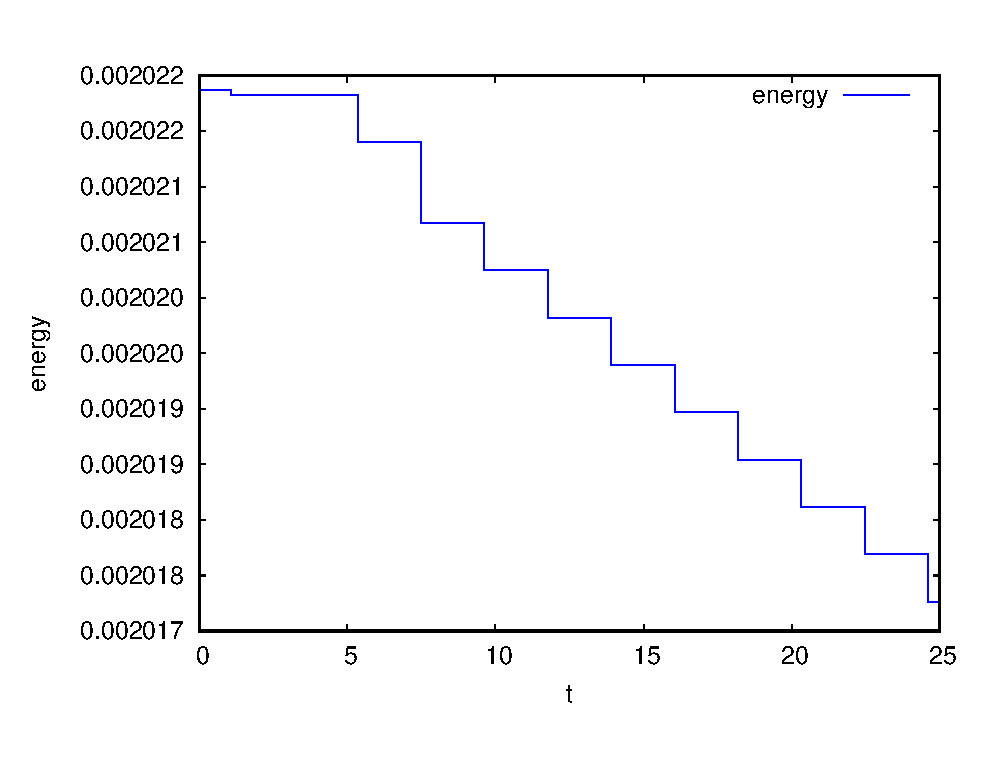
\includegraphics[scale=0.33]{content/pic/self_rot_25/kin_en.eps}
%        \caption{Кинетическая энергия}
%        \label{fig:self_rot_25_kin_en}
%    }
%    \hspace{10pt}
%    \subf{0.3\textwidth}{
%        \centering
%        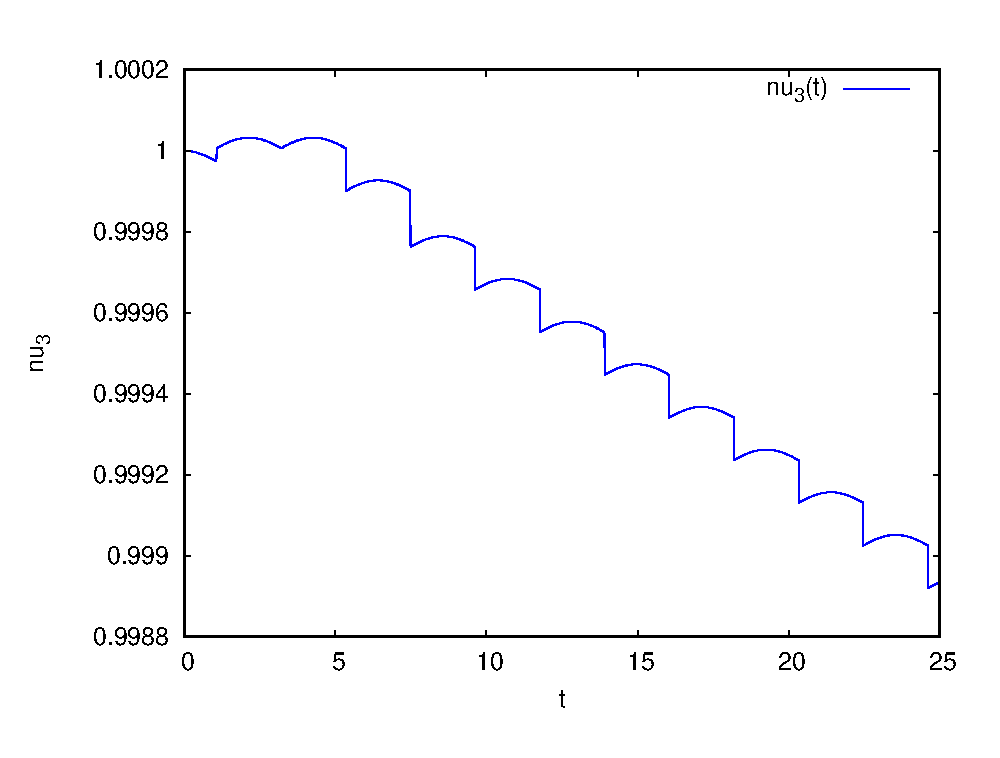
\includegraphics[scale=0.33]{content/pic/self_rot_25/nu3.eps}
%        \caption{Угловая скорость экипажа}
%        \label{fig:self_rot_25_nu3}
%    }
%    \hspace{10pt}
%    \subf{0.3\textwidth}{
%        \centering
%        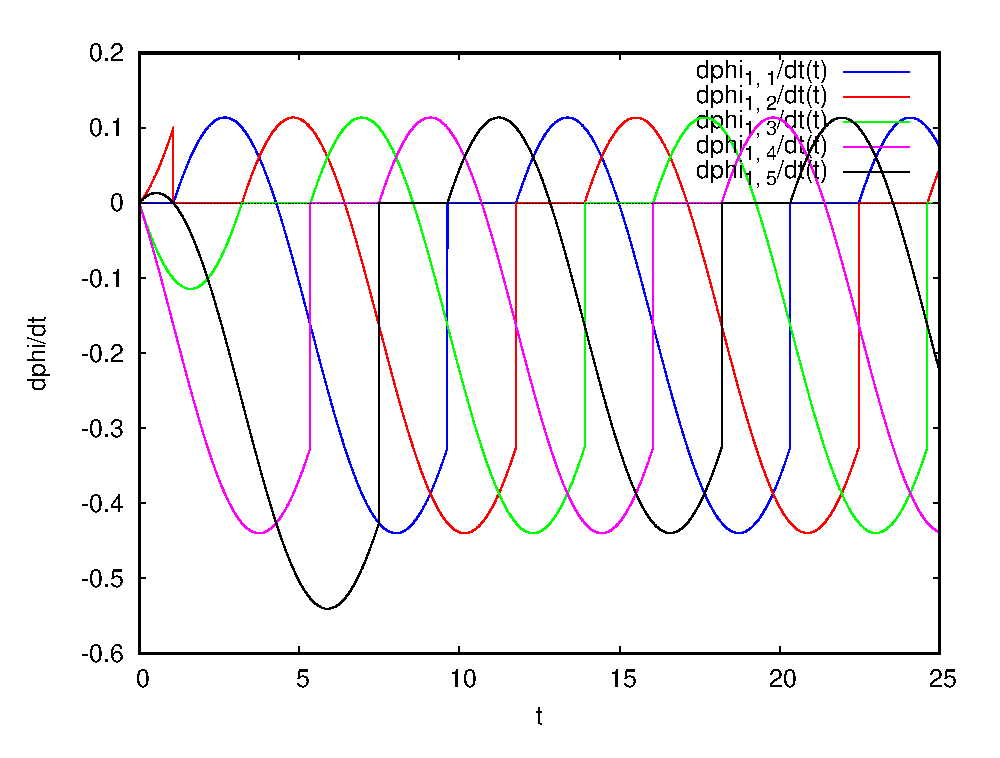
\includegraphics[scale=0.33]{content/pic/self_rot_25/rol_vel.eps}
%        \caption{Угловые скорости роликов}
%        \label{fig:self_rot_25_rol_vel}
%    }
%    \newline
%    \subf{0.3\textwidth}{
%        \centering
%        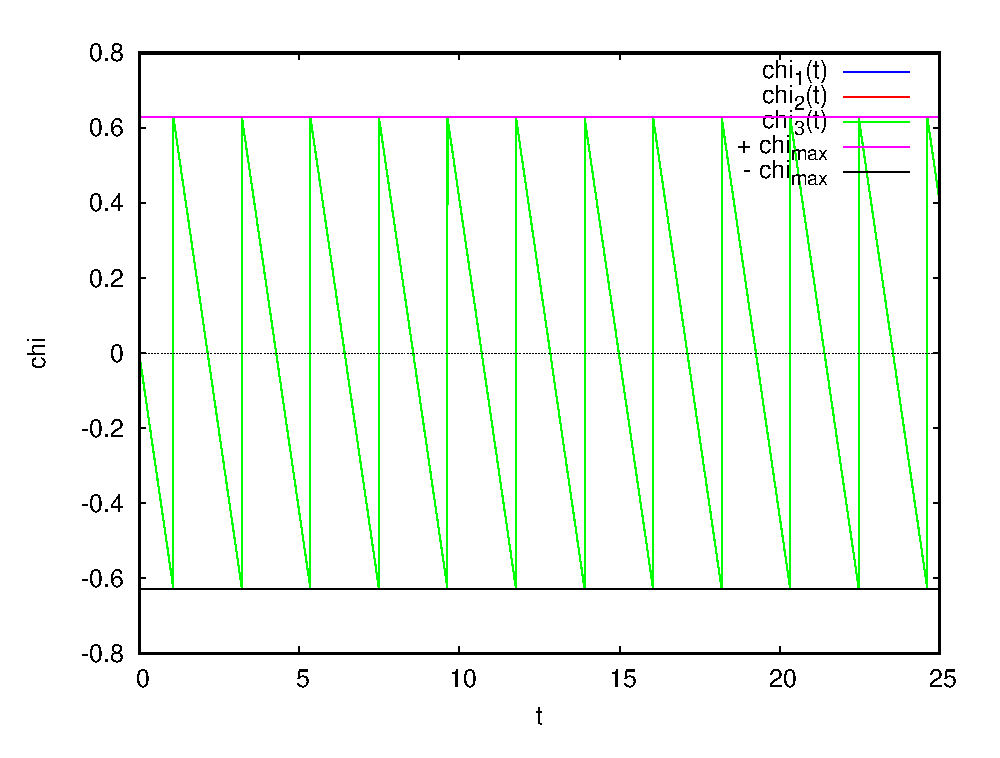
\includegraphics[scale=0.33]{content/pic/self_rot_25/chi.eps}
%        \caption{Углы поворота колес}
%        \label{fig:self_rot_25_chi}
%    }
%    \hspace{10pt}
%    \subf{0.3\textwidth}{
%        \centering
%        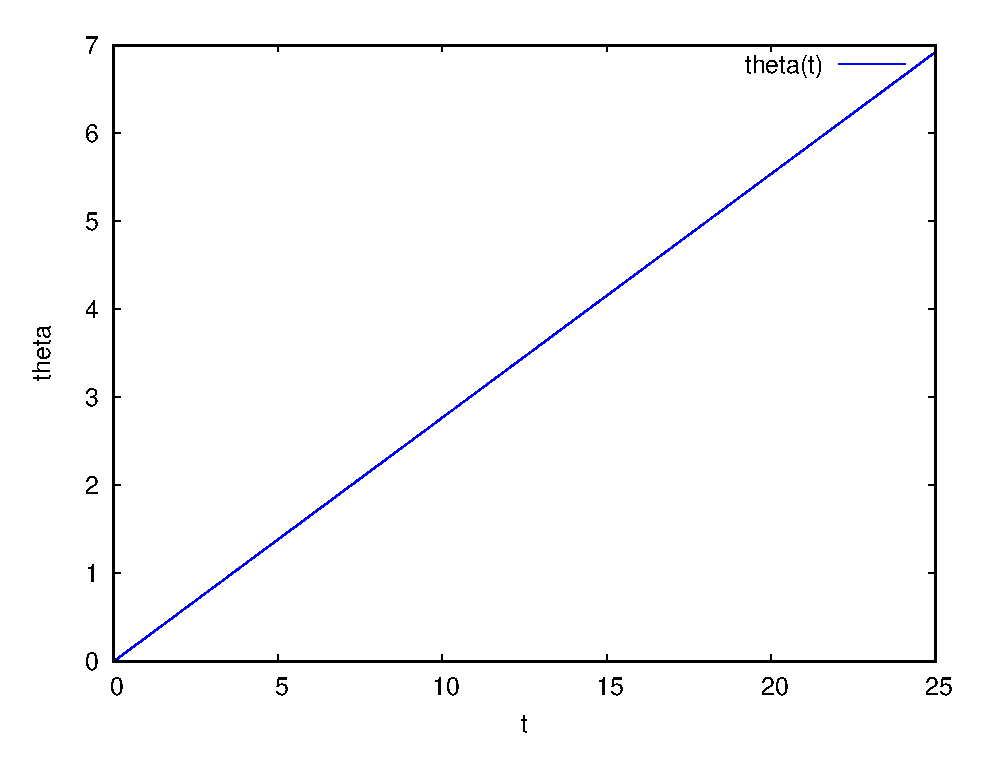
\includegraphics[scale=0.33]{content/pic/self_rot_25/theta.eps}
%        \caption{Угол поворота экипажа}
%        \label{fig:self_rot_25_theta}
%    }
%    \hspace{10pt}
%    \subf{0.3\textwidth}{
%        \centering
%        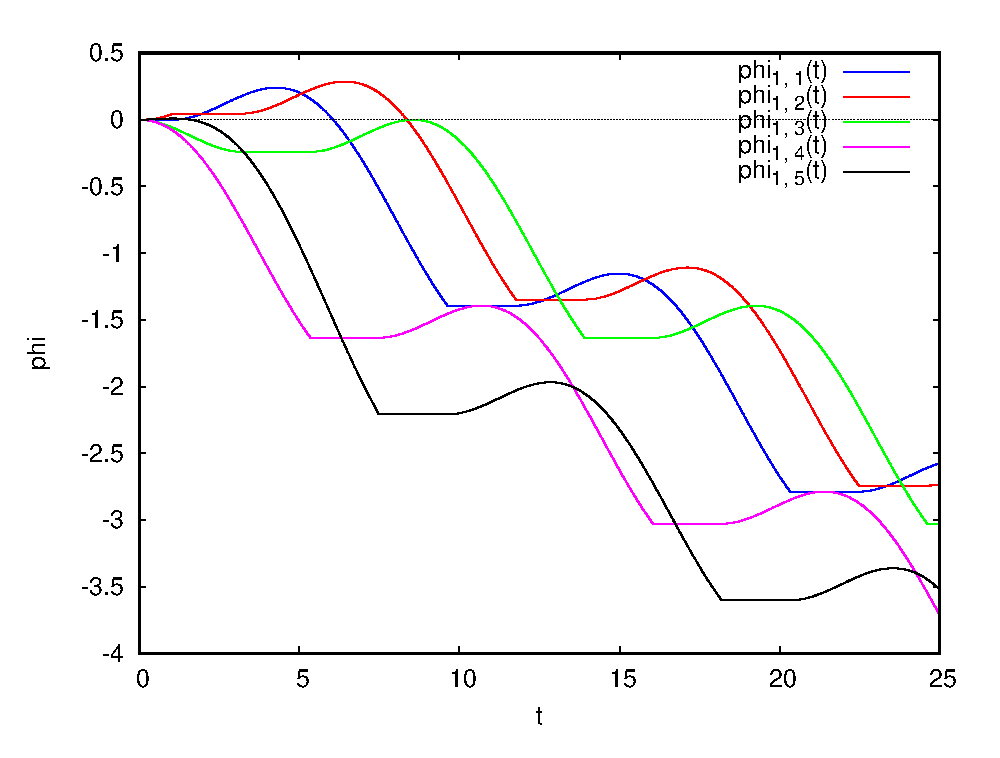
\includegraphics[scale=0.33]{content/pic/self_rot_25/rol_ang.eps}
%        \caption{Углы поворота роликов}
%        \label{fig:self_rot_25_rol_ang}
%    }
%    \caption{Вращение экипажа вокруг своей оси}
%\end{figure}
%\label{fig:self_rot}
%
%\newpage
%
% \subsection{По прямой}
%
%\begin{figure}[h]
%    \hspace{-20pt}
%    \subf{0.22\textwidth}{
%        \centering
%        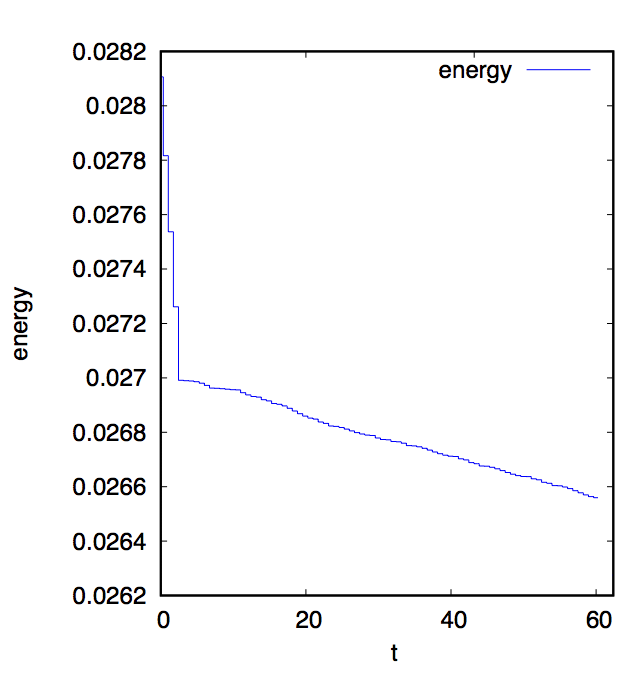
\includegraphics[scale=0.22]{content/pic/straight_60/kin_en.png}
%        \caption{Кинетическая энергия}
%        \label{fig:straight_60_kin_en}
%    }
%    \hspace{20pt}
%    \subf{0.4\textwidth}{
%        \centering
%        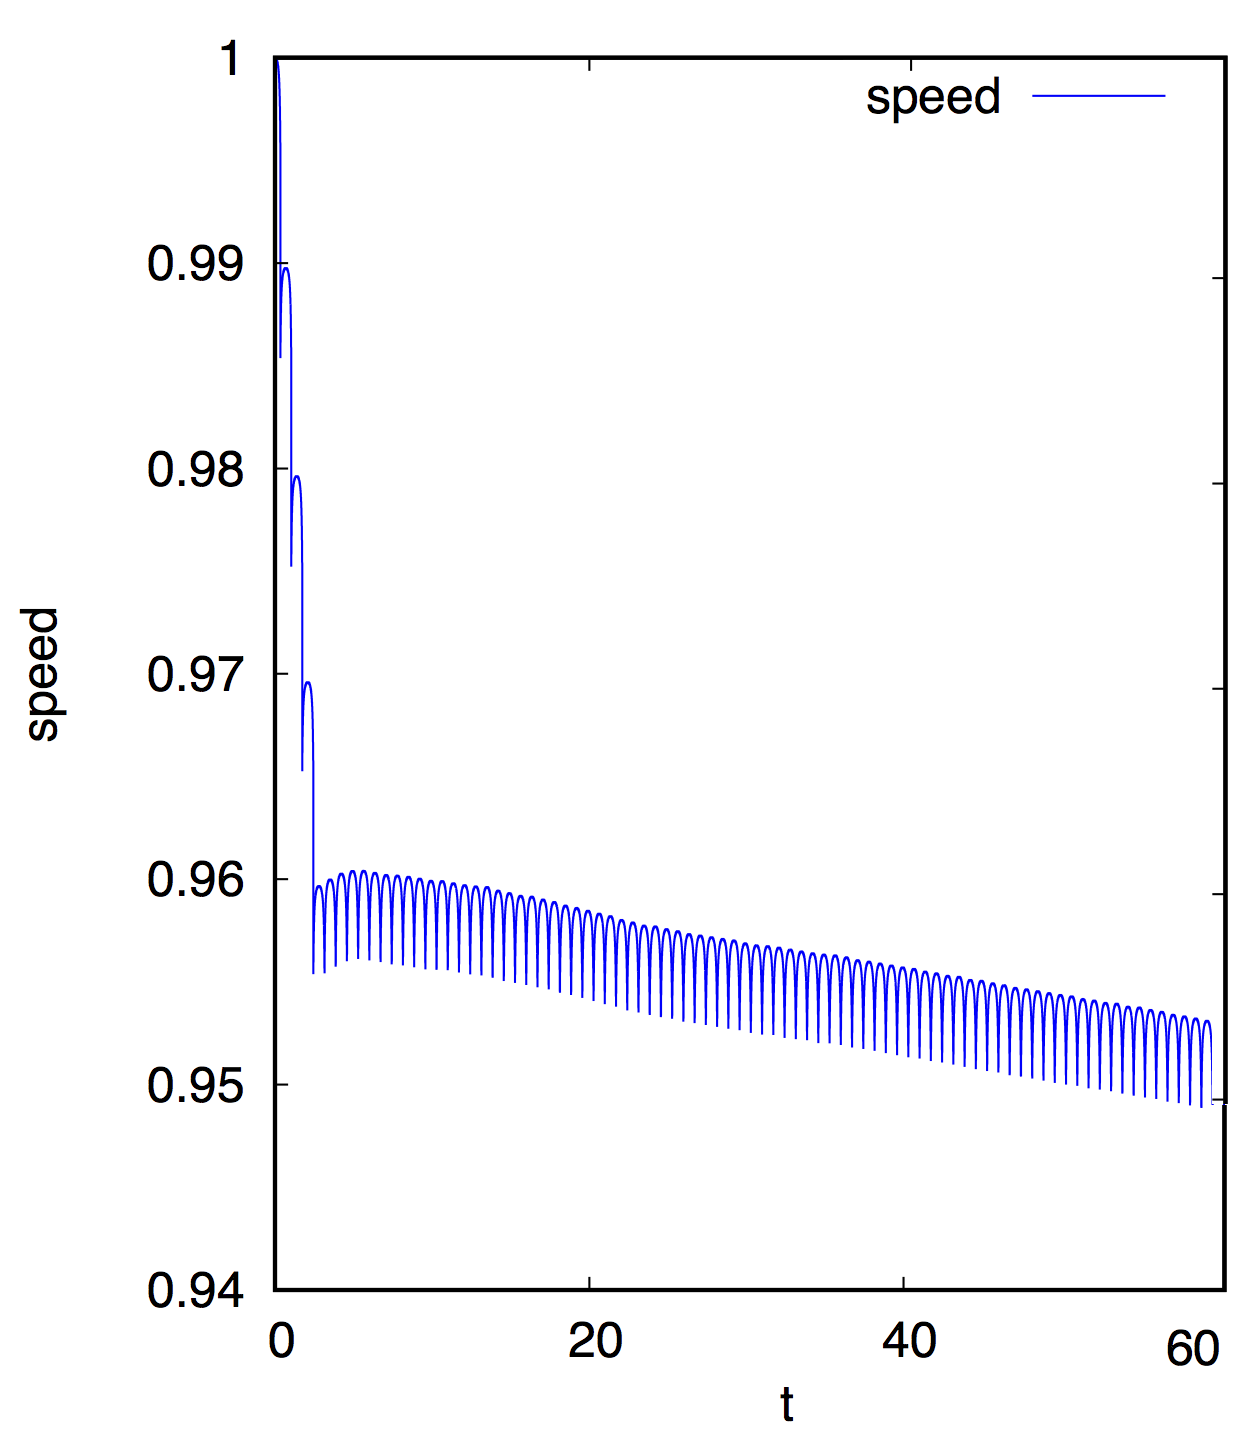
\includegraphics[scale=0.43]{content/pic/straight_60/v.png}
%        \caption{Скорость центра масс}
%        \label{fig:straight_60_v}
%    }
%    % \hspace{10pt}
%    \subf{0.35\textwidth}{
%        \centering
%        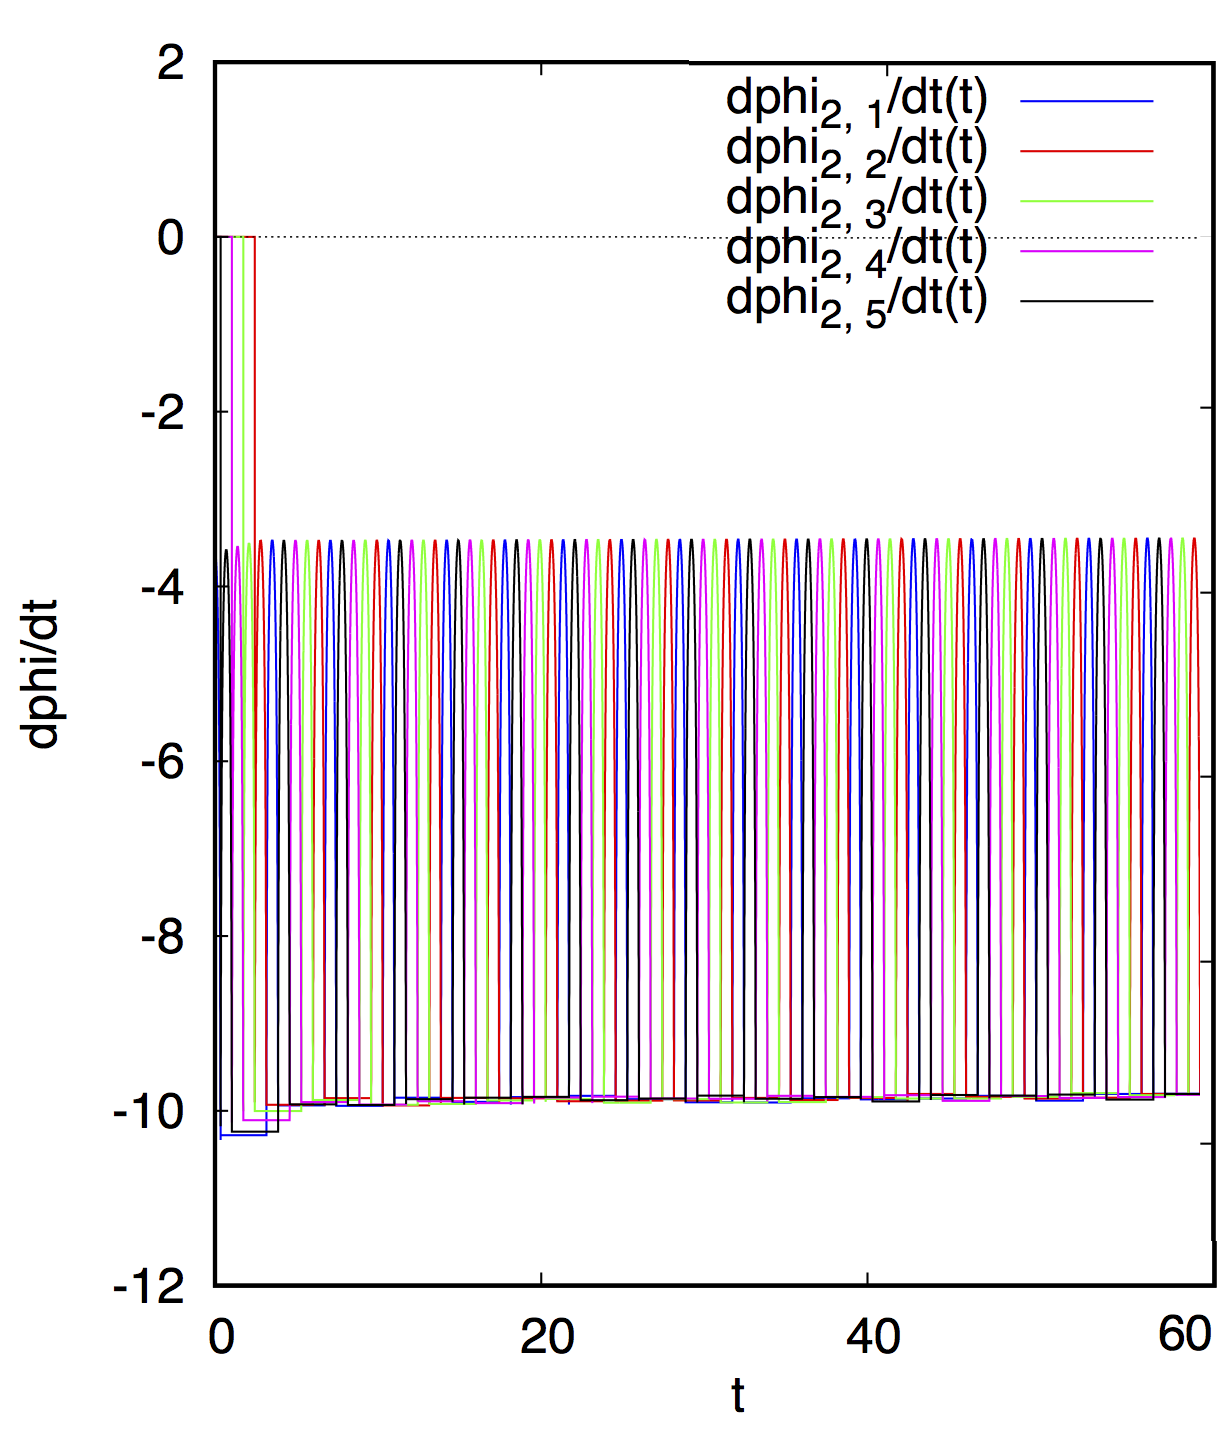
\includegraphics[scale=0.38]{content/pic/straight_60/nus2.png}
%        \caption{Угловые скорости роликов на заднем колесе}
%        \label{fig:straight_60_nus2}
%    }
%    \newline
%    \subf{0.3\textwidth}{
%        \centering
%        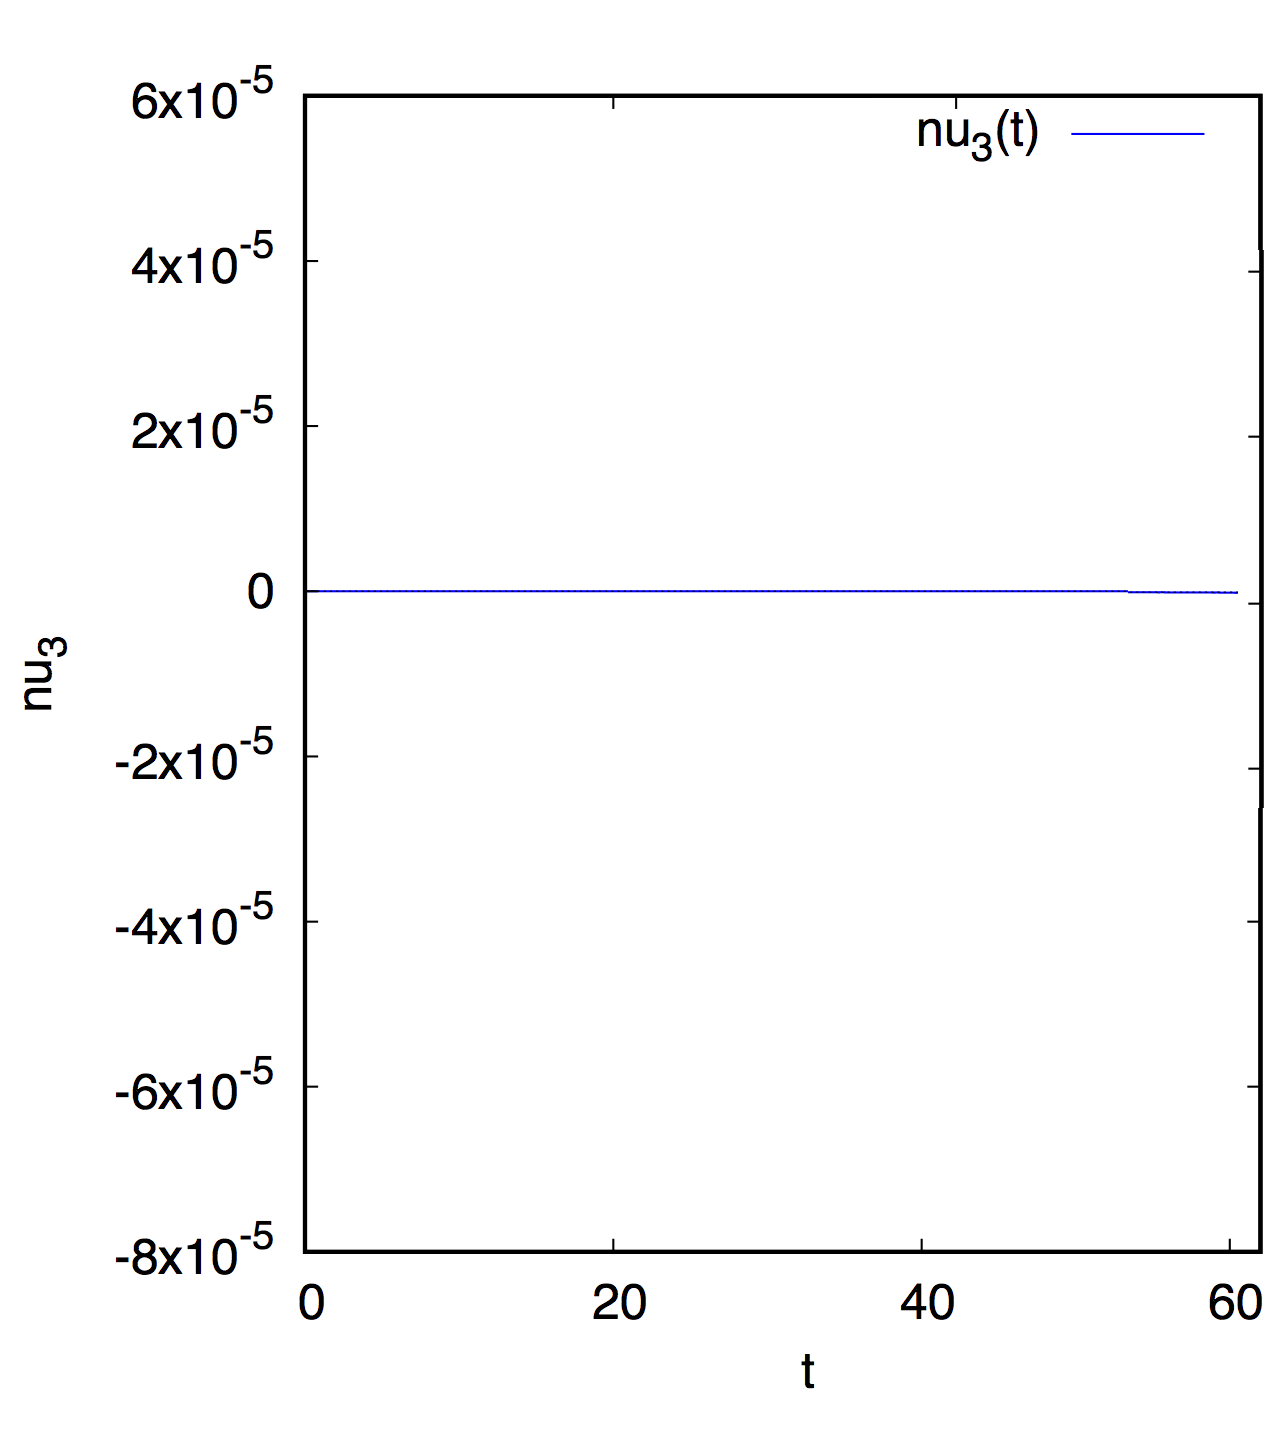
\includegraphics[scale=0.36]{content/pic/straight_60/nu3.png}
%        \caption{Угловая скорость экипажа}
%        \label{fig:straight_60_nu3}
%    }
%    \hspace{10pt}
%    \subf{0.3\textwidth}{
%        \centering
%        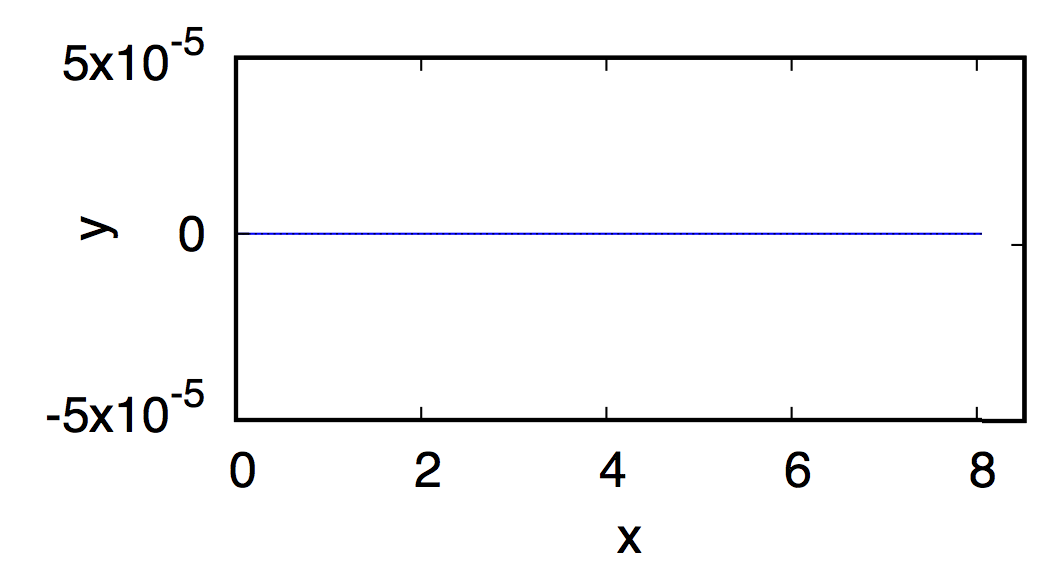
\includegraphics[scale=0.55]{content/pic/straight_60/traj.png}
%        \caption{Траектория}
%        \label{fig:straight_60_traj}
%    }
%    \hspace{10pt}
%    \subf{0.3\textwidth}{
%        \centering
%        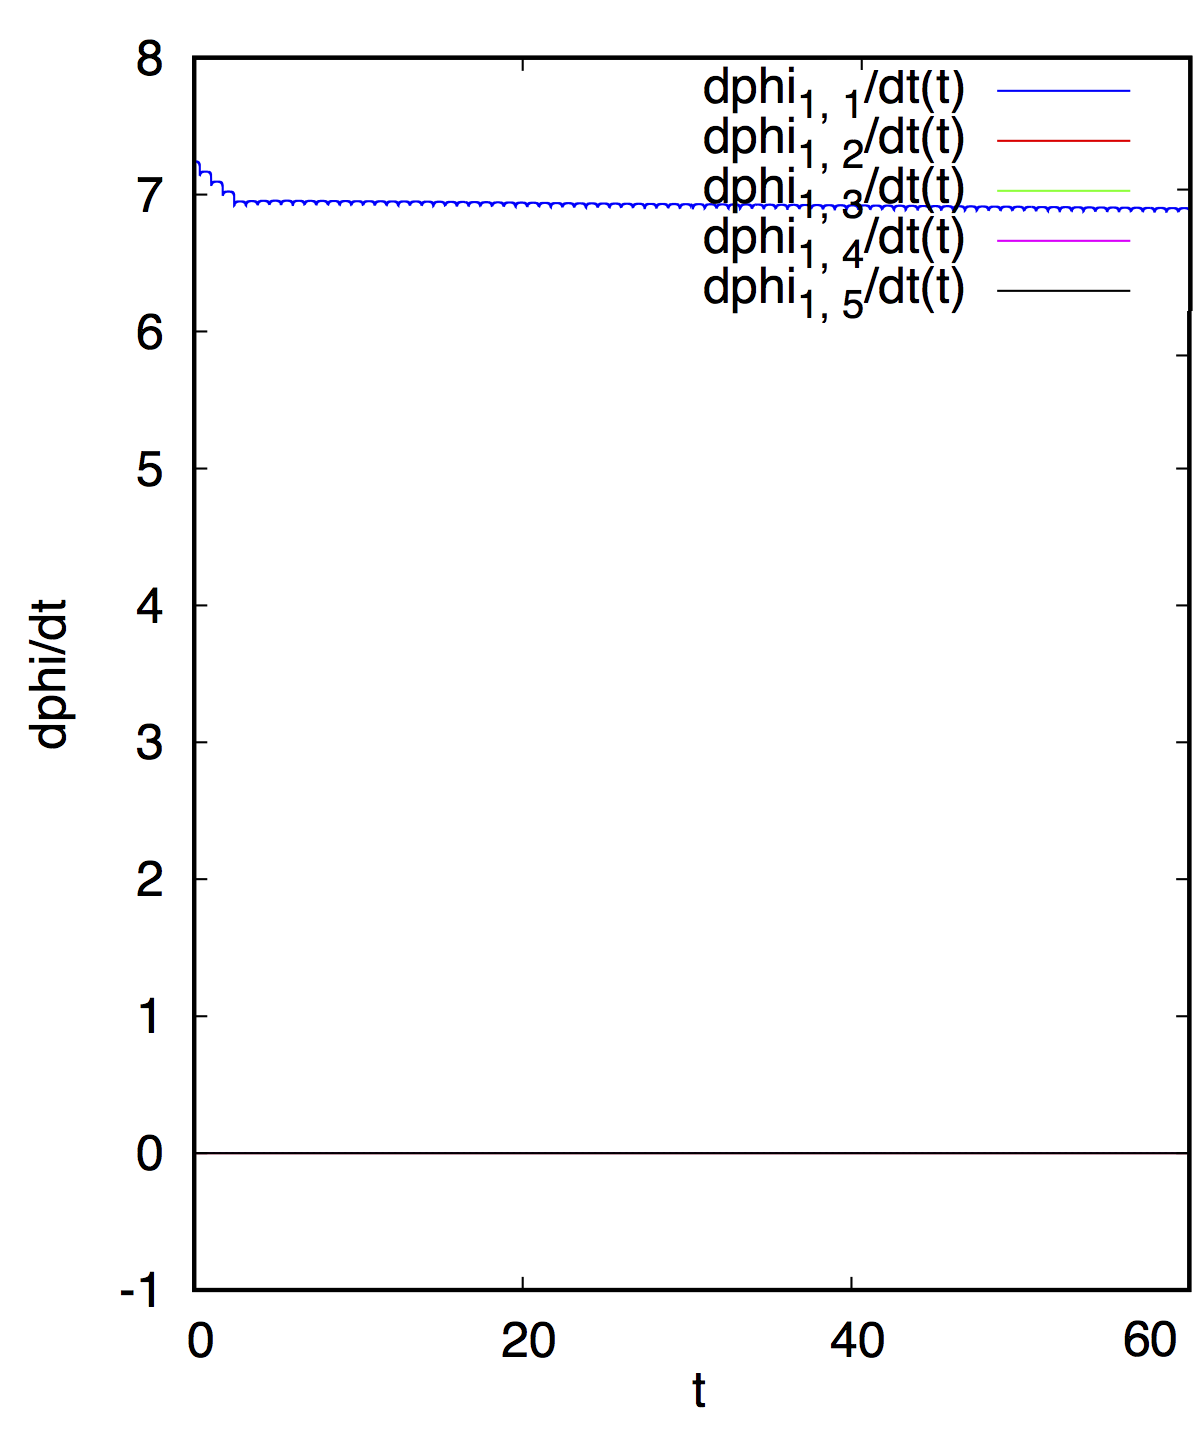
\includegraphics[scale=0.33]{content/pic/straight_60/nus1.png}
%        \caption{Угловые скорости роликов на переднем колесе}
%        \label{fig:straight_60_nus1}
%    }
%    \newline
%    \subf{0.3\textwidth}{
%        \centering
%        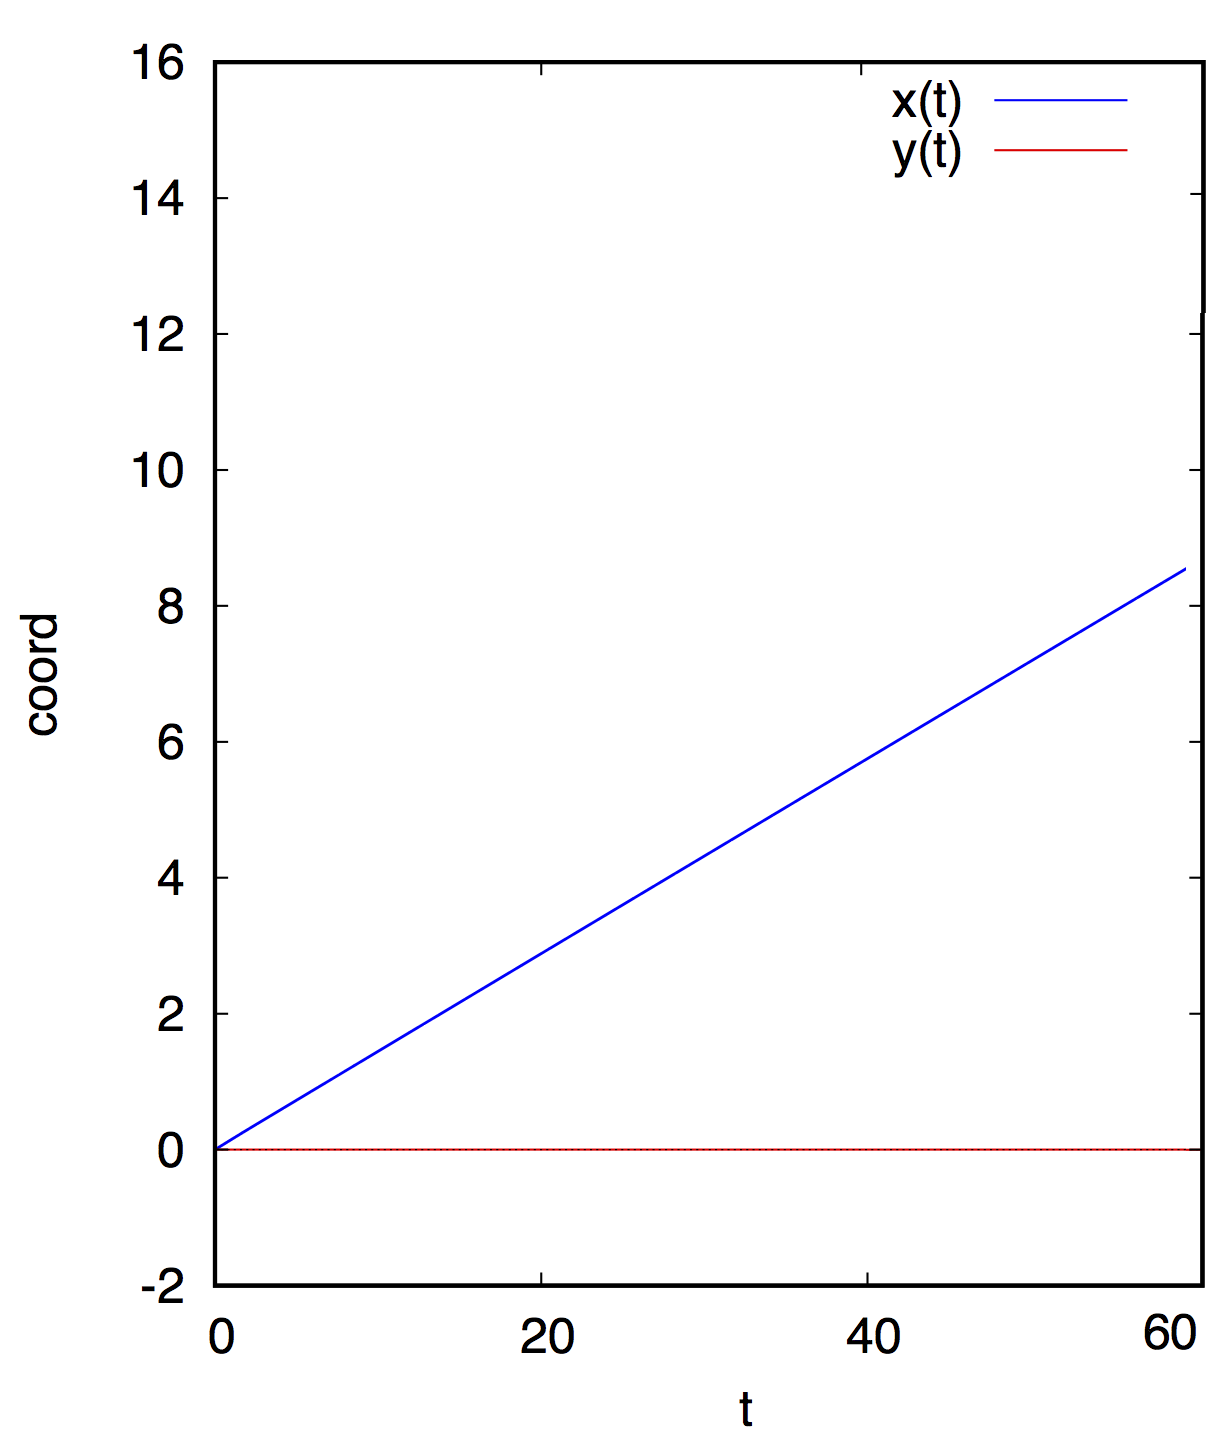
\includegraphics[scale=0.33]{content/pic/straight_60/xy.png}
%        \caption{Координаты центра масс}
%        \label{fig:straight_60_xy}
%    }
%    \hspace{10pt}
%    \subf{0.3\textwidth}{
%        \centering
%        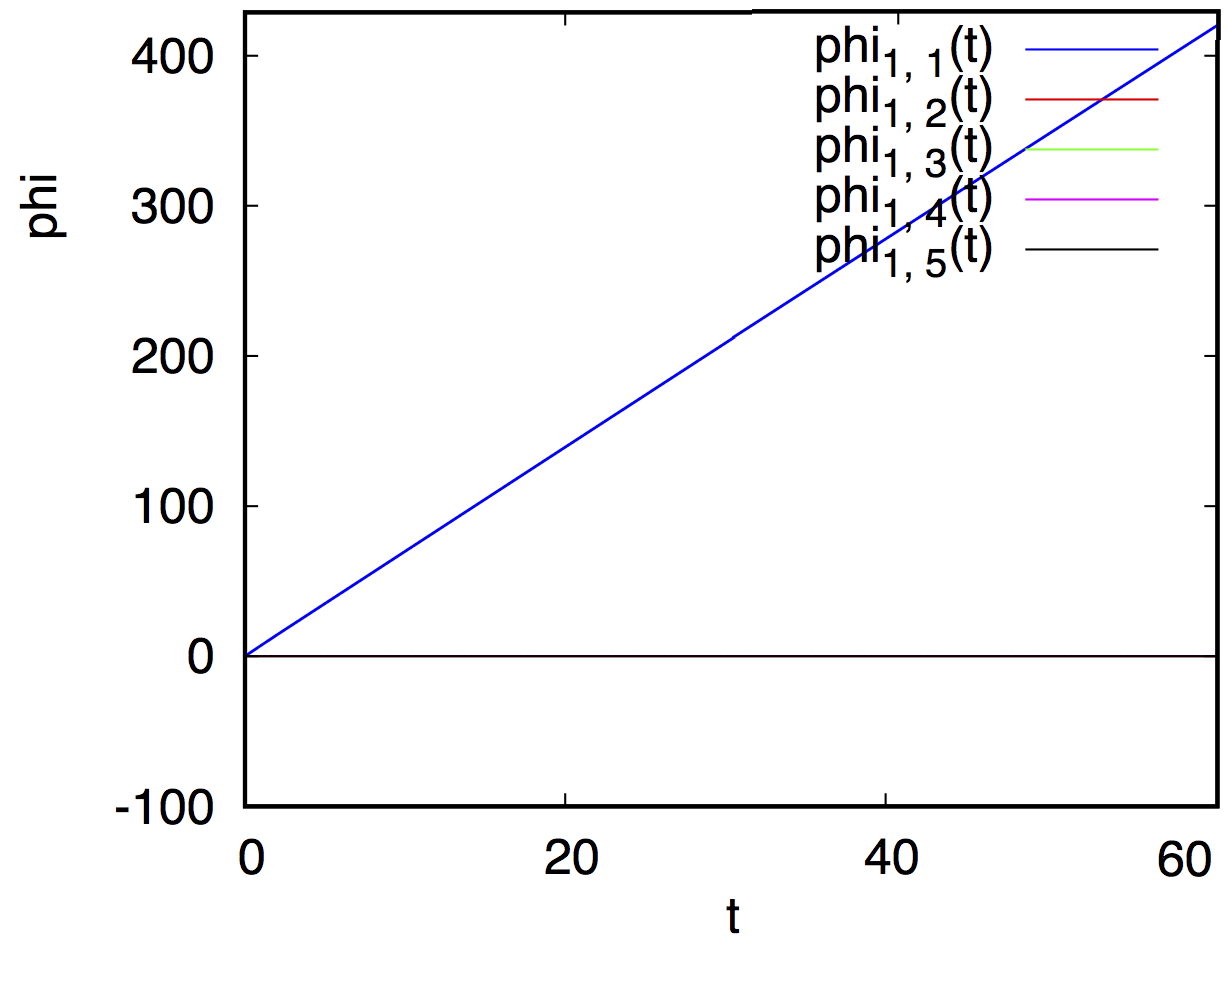
\includegraphics[scale=0.43]{content/pic/straight_60/phi1.png}
%        \caption{Углы поворота роликов на переднем колесе}
%        \label{fig:straight_60_phi1}
%    }
%    \hspace{10pt}
%    \subf{0.3\textwidth}{
%        \centering
%        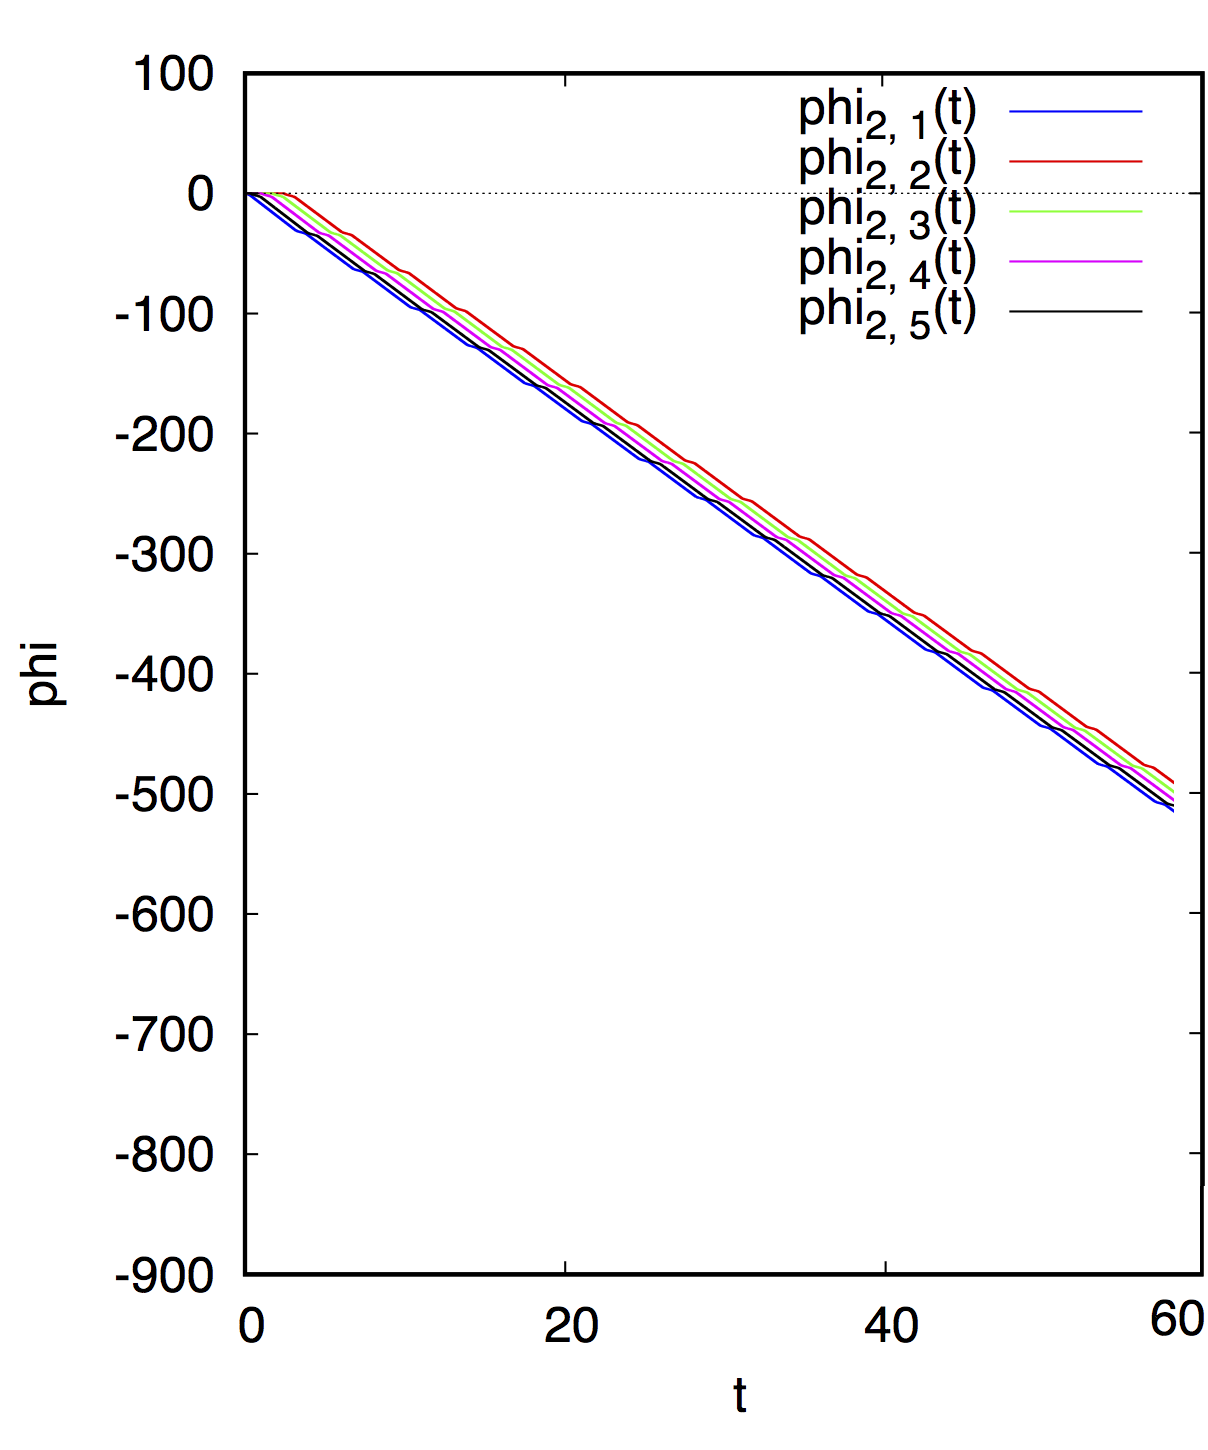
\includegraphics[scale=0.33]{content/pic/straight_60/phi2.png}
%        \caption{Углы поворота роликов на заднем колесе}
%        \label{fig:straight_60_phi2}
%    }
%    \caption{Движение экипажа по прямой}
%\end{figure}
%\label{fig:straight}
%
%\newpage
%
% \subsection{С закруткой}
%
%\begin{figure}[h]
%    \subf{0.3\textwidth}{
%        \centering
%        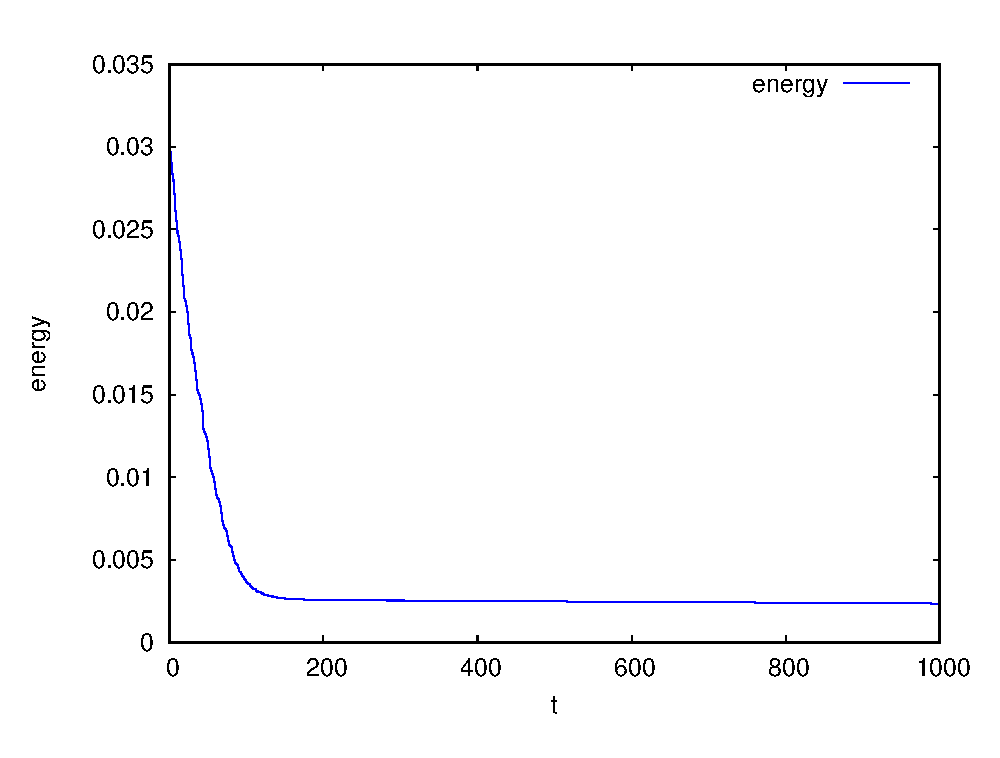
\includegraphics[scale=0.33]{content/pic/wrench_1000/kin_en.eps}
%        \caption{Кинетическая энергия}
%        \label{fig:wrench_1000_kin_en}
%    }
%    \hspace{10pt}
%    \subf{0.3\textwidth}{
%        \centering
%        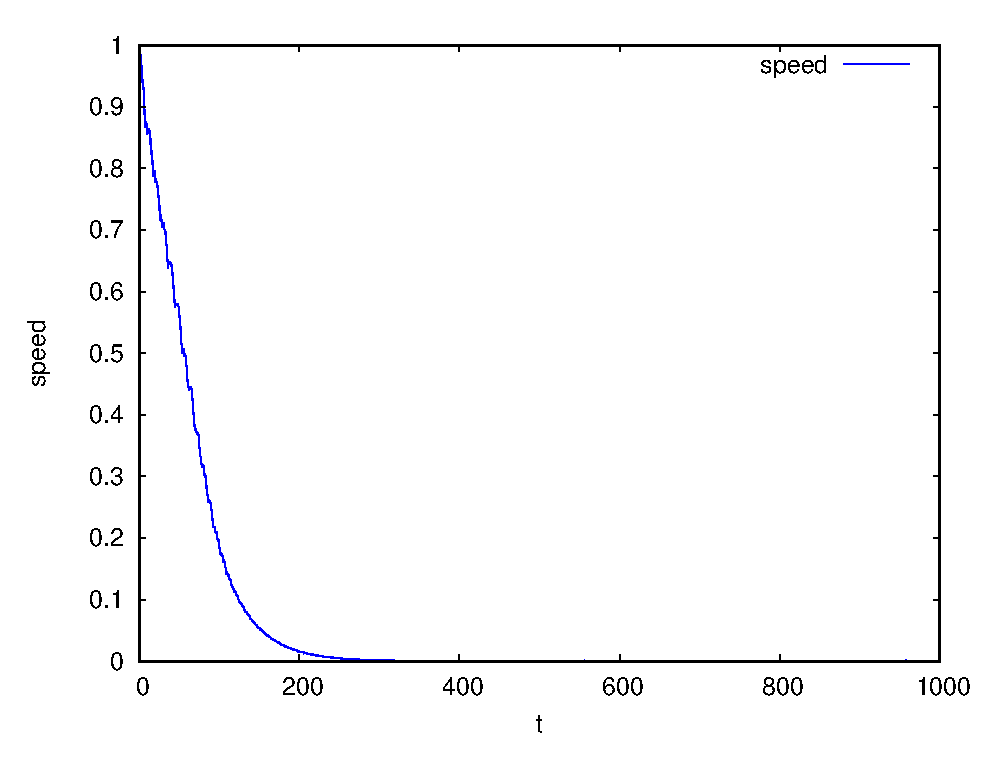
\includegraphics[scale=0.33]{content/pic/wrench_1000/v.eps}
%        \caption{Скорость центра масс}
%        \label{fig:wrench_1000_v}
%    }
%    \hspace{10pt}
%    \subf{0.3\textwidth}{
%        \centering
%        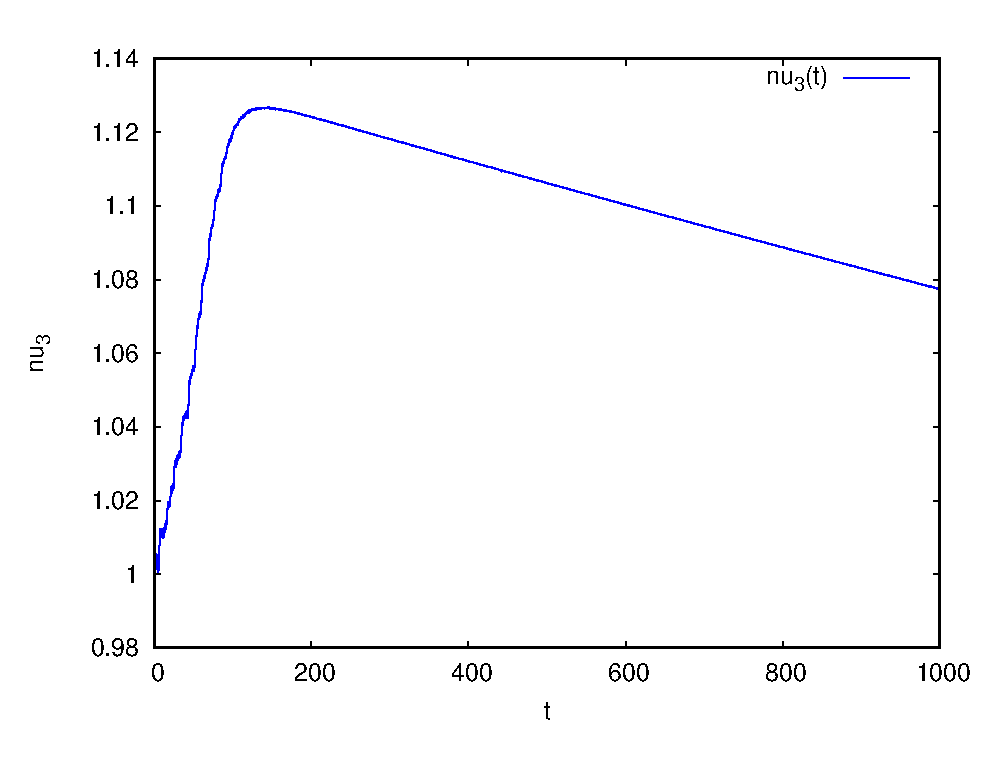
\includegraphics[scale=0.33]{content/pic/wrench_1000/nu3.eps}
%        \caption{Угловая скорость экипажа}
%        \label{fig:wrench_1000_nu3}
%    }
%    \newline
%    \subf{0.45\textwidth}{
%        \centering
%        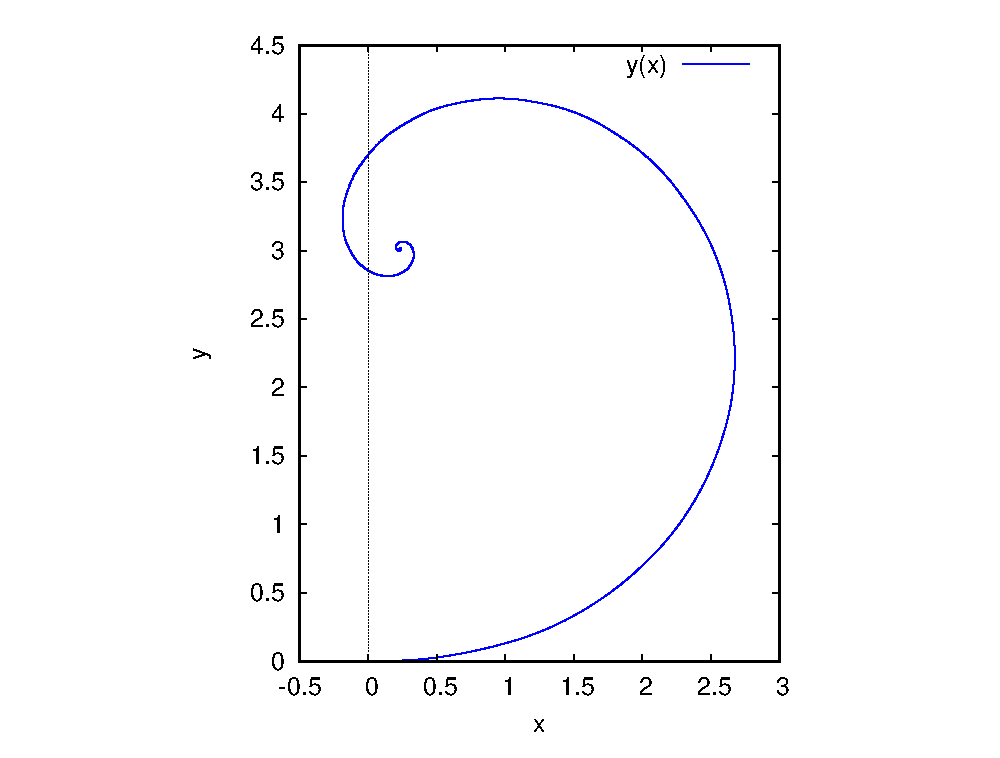
\includegraphics[scale=0.33]{content/pic/wrench_1000/traj.eps}
%        \caption{Траектория центра масс}
%        \label{fig:wrench_1000_traj}
%    }
%    \hspace{10pt}
%    \subf{0.45\textwidth}{
%        \centering
%        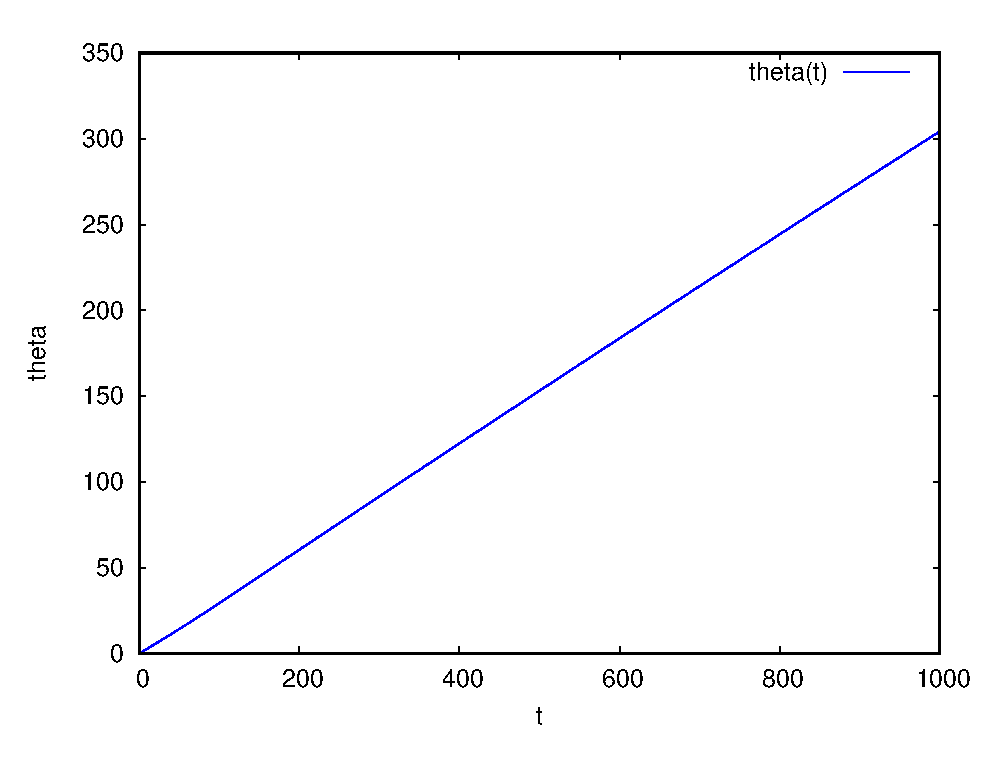
\includegraphics[scale=0.33]{content/pic/wrench_1000/theta.eps}
%        \caption{Угол поворота экипажа}
%        \label{fig:wrench_1000_theta}
%    }
%    \newline
%    \subf{0.45\textwidth}{
%        \centering
%        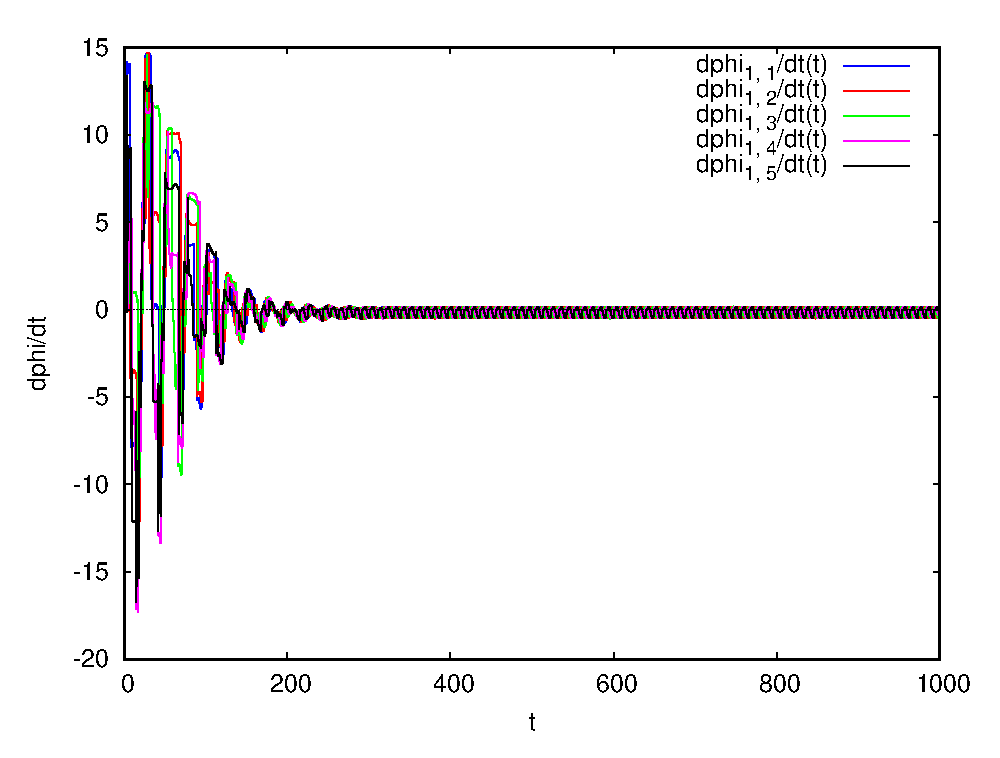
\includegraphics[scale=0.33]{content/pic/wrench_1000/nus1.eps}
%        \caption{Угловые скорости роликов на переднем колесе}
%        \label{fig:wrench_1000_nus1}
%    }
%    \hspace{10pt}
%    \subf{0.45\textwidth}{
%        \centering
%        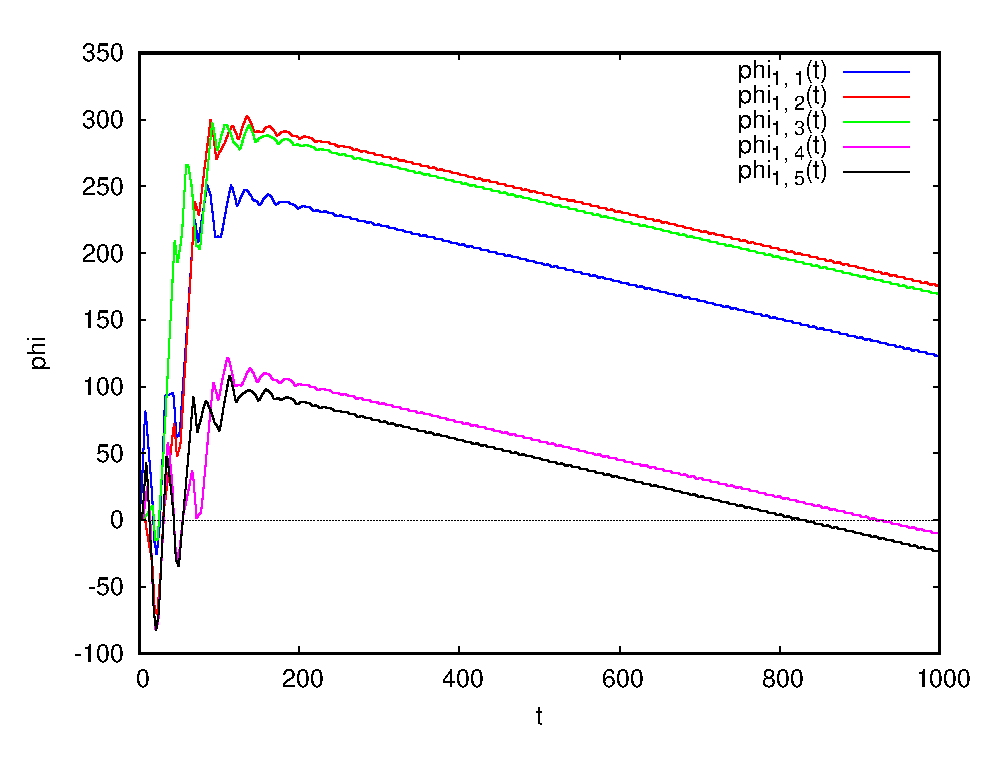
\includegraphics[scale=0.33]{content/pic/wrench_1000/phi1.eps}
%        \caption{Углы поворота роликов на переднем колесе}
%        \label{fig:wrench_1000_phi1}
%    }
%    \caption{Движение экипажа с закруткой}
%\end{figure}
%\label{fig:wrench}
%
